\chapter{Chapter 2: An Overview of x86 Architecture}\label{ch-x86}

\section{Introduction}\label{introduction}

In our situation, and by using modern terminology, we can view the
processor as a \emph{library} and \emph{framework}. A library because it
provides us with a bunch of instructions to perform whatever we want,
and a framework because it has general rules that organize the overall
environment of execution, that is, it forces us to work in a specific
way. We have seen some aspects of the first part when we have written
the bootloader, that is, we have seen the processor as a library. In
this chapter, we are going to see how the processor works as a framework
by examining some important and basic concepts of x86. We need to
understand these concepts to start the real work of writing 539kernel.

\section{x86 Operating Modes}\label{x86-operating-modes}

In x86 an operating mode specifies the overall picture of the processor,
such as the maximum size of available registers, the available advanced
features for the running operating system, the restrictions and so on.

When we developed the bootloader in the previous chapter we have worked
with an x86 operating mode named \emph{real address mode} (or for short
\emph{real mode}) which is an old operating mode that is still supported
by modern x86 processors for the sake of backward compatibility, due to
that when the computer is turned on, it initially runs on real mode.

Real mode is a \lstinline!16-bit! operating mode which means that,
maximally, only \lstinline!16! bits of register size can be used, even
if the actual size of the registers is 64-bit. Using only \lstinline!16!
bits of registers has consequences other than the size itself, these
consequences are considered as disadvantages in modern days, for
example, in real mode the size of the main memory is limited, even if
the computer has 16GB of memory, real mode can deal only with 1MB.
Furthermore, any code which runs on real mode should be a
\lstinline!16-bit! code, for example, the aforementioned
\lstinline!32-bit! registers (such as \lstinline!eax!) cannot be used in
real mode code, their \lstinline!16-bit! counterparts should be used
instead, as an example, the 16-bit \lstinline!ax! should be used instead
of \lstinline!eax! and so on.

Some core features of modern operating systems nowadays are:
multitasking, memory protection and virtual memory \footnote{If some of
  these terms are new for you don't worry about them too much, you will
  learn them gradually throughout this book.} and real mode provides
nothing to implement these features. However, in modern x86 processors,
new and more advanced operating modes have been introduced, namely,
\emph{protected mode} which is a \lstinline!32-bit! operating mode and
\emph{long mode} which is a relatively new \lstinline!64-bit! operating
mode. Although the long mode provides more capacity for its users, for
example, it can deal with 16 \textbf{exabytes} of memory, we are going
to focus on protected mode since it provides the same basic mechanisms
that we need to develop a modern operating system kernel with the
aforementioned features, hence, 539kernel is a \lstinline!32-bit! kernel
which runs under protected mode.

Since protected mode is a \lstinline!32-bit! operating mode then
\lstinline!32! bits of registers can be used, also, protected mode has
the ability to deal with \lstinline!4GB! of main memory, and most
importantly, it provides important features which we are going to
explore through this book that helps us in implementing modern operating
system kernel features.

As we have said before, \emph{multitasking} is one of core features that
modern operating systems provide. In multitasking environment more than
one software can run at the same time, at least illusionary, even if
there is only one processor or the current processor has only one core.
For the sake of making our next discussion easier we should define the
term \emph{process} which means a program that is currently running. For
example, if your web browser is currently running then this running
instance of it is called a process, its code is loaded into the main
memory and the processor is currently executing it. Another property of
general-purpose operating systems is that they allow the user to run any
software from unknown sources which means that these software cannot be
trusted, they may contain code that intentionally or even
unintentionally breach the security of the system or cause the system to
crash.

Due to these two properties of modern general-purpose operating systems,
the overall system needs to be protected from multiple actions.
\textbf{First}, either in multitasking or monotasking \footnote{That is,
  the user of the operating system can only run one process at a given
  time. DOS is a an example of monotasking operating system.}
environment, the kernel of the operating system which is the most
sensitive part of the system, should be protected from current
processes, no process should be able to access any part of the kernel's
memory either by reading from it or writing to it, also, no process
should be able to call any of kernel's code without kernel's consent.
\textbf{Second}, the sensitive instructions and registers that change
the behavior of the processor (e.g.~switching from real-mode to
protected-mode) should be only allowed for the kernel which is the most
privileged component of the system, otherwise, the stability of the
system will be in danger. \textbf{Third}, in multitasking environment
the running processes should be protected from each other in the same
way the kernel is protected from them, no process should interfere with
another.

In x86, the \emph{segmentation} mechanism provided a logical view of
memory in real-mode and it has been extended in protected-mode to
provide the needed protection which has been described in the third
point \footnote{Segmentation will be examined in details later on this
  chapter.}, while segmentation can be used in x86 for this kind of
protection, it is not the sole way to perform that, the another
well-known way is called \emph{paging}, but segmentation is the default
in x86 and cannot be turned off while paging is optional, the operating
system has the option to use it as a way of memory protection or not.

Also, in the protected-mode the concept of \emph{privilege levels} has
been introduced to handle the protections needed in the previous first
and second points. The academic literature of operating systems separate
the system environment into two modes, \emph{kernel-mode} and
\emph{user-mode}, at a given time, the system may run on one of these
modes and not both of them. The kernel runs on kernel-mode, and has the
privilege to do anything (e.g.~access any memory location, access any
resource of the system and perform any operation), while the user
applications run on user-mode which is a restricted environment where
the code that runs on doesn't have the privilege to perform sensitive
actions.

This kind of separation has been realized through privilege levels in
x86 which provides \textbf{four privilege levels} numbered from
\lstinline!0! to \lstinline!3!. The privilege level \lstinline!0! is the
most privileged level which can be used to realize the kernel-mode while
the privilege level \lstinline!3! is the least privileged which can be
used to realize the user-mode. For privilege levels \lstinline!1! and
\lstinline!2! it's up to the kernel's designer to use them or not, some
kernel designs suggest to use these levels for device drivers. According
to Intel's manual, if the kernel's design uses only two privilege
levels, that is, a kernel-mode and user-mode, then the privilege level
\lstinline!0! and \lstinline!3! should be used and not for example
\lstinline!0! and \lstinline!1!.

In addition to protecting the kernel's code from being called without
its consent and protecting kernel's data from being accessed by user
processes (as both required by first point above), the privilege levels
also prevent user processes \footnote{That is, the processes which runs
  on privilege level greater than \lstinline!0!} from executing
\emph{privileged instructions} (as required by second point above), only
the code which runs in the privilege level \lstinline!0!, that is, the
kernel, will be able to execute these instructions since they could
manipulate sensitive parts of the processor's environment \footnote{For
  example, loading \lstinline!GDT! register by using the instruction
  \lstinline!lgdt! as we will see later in this chapter.} that only the
kernel should maintain.

When a system uses different privilege levels to run, as in most modern
operating systems, the x86 processor maintains what is called
\emph{current privilege level} (CPL) which is, as its name suggests, the
current privilege level of the currently running code. For example, if
the currently running code belongs to the kernel then the current
privilege level will be \lstinline!0! and according to it, the processor
is going to decide allowed operations. In other words, we can say that
the processor keeps tracking the current state of the currently running
system and one of the information in this state is in which privilege
level (or mode) the system is currently running.

\section{Numbering Systems}\label{numbering-systems}

The processor works with all values as \emph{binary numbers} while it is
natural for us as human beings to deal with numbers as \emph{decimal
numbers}. A number by itself is an abstract concept, it is something in
our mind, but to communicate with each others, we represent the numbers
by using symbols which is named \emph{numerals}. For example, the
conceptual number \lstinline!one! can be represented by different
\emph{numeral systems}. In Arabic numeral system the number
\lstinline!one! is expressed as \lstinline!1!, while in Roman numeral
system it is expressed as \lstinline!I!.

A numeral system is \emph{writing system}, that is, it gives us rules of
how to write a number down as a symbol, it focuses on the way of writing
the numbers. On the other hand, the numbers can be dealt with by a
\emph{numbering system}, we use the \emph{decimal numbering system} to
deal with numbers, think about them and perform arithmetic operations
upon them, the processor uses the \emph{binary numbering system} to do
the same with numbers. There are numbering systems other than the
decimal and binary numbering system, and any number can be represented
by any numbering system.

A number system is defined by its \emph{base} which is also called
\emph{radix}, this base defines the list of available \emph{digits} in
the numbering system starting from \lstinline!0! to
\lstinline!base - 1!, the total of available digits equals the base.
Consider the decimal numbering system, its base is \lstinline!10! which
means the available digits in this system are:
\lstinline!0, 1, 2, 3, 4, 5, 6, 7, 8, 9!, a total of \lstinline!10!
digits. These digits can be used to create larger numbers, for example,
\lstinline!539! which consists of the digits \lstinline!5!,
\lstinline!3! and \lstinline!9!.

On the other hand, the base of binary numbering system is \lstinline!2!,
therefore, the available digits are only \lstinline!0! and
\lstinline!1!, and as in the decimal numbering system they can be used
to compose larger numbers, for example, the number \lstinline!two! in
binary numbering system is \lstinline!10! \footnote{And from here came
  the well-known joke: ``There are 10 types of people in this world,
  those who understand binary and those who don't''.}, be careful, this
numeral does not represent the number \lstinline!ten!, it represents the
number \lstinline!two! but in binary numbering system. When we discuss
numbers in different numbering systems, we put the initial letter of the
numbering system name in the end of the number, for example,
\lstinline!10d! and \lstinline!10b! are two different numbers, the first
one is \lstinline!ten! in \textbf{d}ecimal while the second one is
\lstinline!two! in \textbf{b}inary.

Furthermore, basic arithmetic operations such as addition and
subtraction can be performed on the numbering system, for example, in
binary \lstinline!1 + 1 = 10! and it can be performed systematically,
also, a representation of any number in any numbering system can be
converted to any other numbering system systematically \footnote{I think
  It's too brave to state this claim, however, it holds true at least
  for the well-known numbering system.}, while this is not a good place
to show how to perform the operations and conversions for different
numbering system, you can find many online resources that explain these
operations on the well-known number systems.

By now it should be obvious for you that changing the base (radix) gives
us a new numbering system and the base can be any number which implies
that the total of numbering systems is infinite! One of useful and
well-known numbering system is \emph{hexadecimal} which its base is
\lstinline!16! and its digits are
\lstinline!0, 1, 2, 3, 4, 5, 6, 7, 8, 9, A, B, C, D, E, F! where
\lstinline!A! means \lstinline!ten!, \lstinline!B! means
\lstinline!eleven! and so on. So, why hexadecimal is useful in our
situation? Since binary is used in the processor it will be easier to
discuss some related entities such as the value of \lstinline!FLAGS!
register which each bit on it represents a value for a different thing,
another example is memory addresses. But consider the following example
which is a binary number that represents a memory address.

\begin{lstlisting}
00000000 00000000 00000000 00000001b
\end{lstlisting}

It is too long and it will be tedious to work with, and for that the
hexadecimal numbering system can be useful. Each digit in hexadecimal
represents \textbf{four} bits \footnote{Can you tell why? {[}Hint: How
  the maximum hexadecimal number \lstinline!F! is represented in
  binary?{]}}, that is, the number \lstinline!0h! in
\textbf{h}exadecimal is equivalent to \lstinline!0000b! in binary. As
the \lstinline!8 bits! known as a byte, the \lstinline!4 bits! is known
as a \emph{nibble}, that is, a nibble is a half byte and, as we have
said, but in other words, one digit of hexadecimal represents a nibble.
So, we can use hexadecimal to represent the same memory address value in
more elegant way.

\begin{lstlisting}
00 00 00 01h
\end{lstlisting}

\begin{longtable}[]{@{}lll@{}}
\caption{An Example of How Zero to Fifteen are Represented in the Three
Numbering Systems.}\tabularnewline
\toprule
Decimal & Binary & Hexadecimal\tabularnewline
\midrule
\endfirsthead
\toprule
Decimal & Binary & Hexadecimal\tabularnewline
\midrule
\endhead
0 & 0 & 0\tabularnewline
1 & 1 & 1\tabularnewline
2 & 10 & 2\tabularnewline
3 & 11 & 3\tabularnewline
4 & 100 & 4\tabularnewline
5 & 101 & 5\tabularnewline
6 & 110 & 6\tabularnewline
7 & 111 & 7\tabularnewline
8 & 1000 & 8\tabularnewline
9 & 1001 & 9\tabularnewline
10 & 1010 & A\tabularnewline
11 & 1011 & B\tabularnewline
12 & 1100 & C\tabularnewline
13 & 1101 & D\tabularnewline
14 & 1110 & E\tabularnewline
15 & 1111 & F\tabularnewline
\bottomrule
\end{longtable}

\section{The Basic View of Memory}\label{the-basic-view-of-memory}

The basic view of the main memory is that it is an \emph{array of
cells}, each cell has the ability to store one byte and it is reachable
by a unique number called \emph{memory address} \footnote{The
  architecture which each memory address points to \lstinline!1 byte! is
  known as \emph{byte-addressable architecture} or \emph{byte machines}.
  It is the most common architecture. Of course, other architectures are
  possible, such as \emph{word-addressable architecture} or \emph{word
  machines}.}, the range of memory addresses starts from \lstinline!0!
to some limit \lstinline!x!, for example, if the system has
\lstinline!1MB! of \emph{physical} main memory, then the last memory
address in the range will be \lstinline!1023!, as we know,
\lstinline!1MB! = \lstinline!1024 bytes! and since the range starts from
\lstinline!0! and not \lstinline!1!, then the last memory address in
this case is \lstinline!1023! and not \lstinline!1024!. This range of
memory addresses is known as \emph{address space} and it can be a
\emph{physical address space} which is limited by the physical main
memory or a \emph{logical address space}. A well-known example of using
logical address space that we will discuss in a latter chapter is
\emph{virtual memory} which provides a logical address space of size
\lstinline!4GB! in \lstinline!32-bit! architecture even if the actual
size of physical main memory is less than \lstinline!4GB!. However, The
address space starts from the memory address \lstinline!0!, which is the
index of the first cell (byte) of the memory, and it increases by
\lstinline!1!, so the memory address \lstinline!1! is the index of the
second cell of the memory, \lstinline!2! is the index of third cell of
memory and so on. Viewing the memory as an array of contiguous cells is
also known as \emph{flat memory model}.

\begin{figure}
\centering
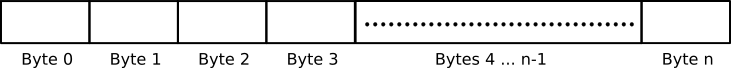
\includegraphics[width=0.75000\textwidth]{Figures/x86-ch/memory-physical-view.png}
\caption{The Physical View of the Memory. The Size of it is
\lstinline!n! Bytes.}\label{fig:memory_physical_view}
\end{figure}

When we say \emph{physical} we mean the actual hardware, that is, when
the maximum capacity of the hardware of the main memory (RAM) is
\lstinline!1MB! then the physical address space of the machine is up to
\lstinline!1MB!. On the other hand, when we say \emph{logical} that
means it doesn't necessarily represents or obeys the way the actual
hardware works on, instead it is a hypothetical way of something that
doesn't exist in the real world (the hardware). To make the
\emph{logical} view of anything works, it should be mapped into the real
\emph{physical} view, that is, it should be somehow translated for the
physical hardware to be understood, this mapping is handled by the
software or sometimes special parts of the hardware.

Now, for the following discussion, let me remind you that the memory
address is just a numerical value, it is just a number. When I discuss
the memory address as a mere number I call it \emph{memory address
value} or \emph{the value of memory address}, while the term
\emph{memory address} keeps its meaning, which is a unique identifier
that refers to a specific location (cell) in the main memory.

The values of memory addresses are used by the processor all the time to
be able to perform its job, and when it is executing some instructions
that involve the main memory (e.g.~reading a content from some memory
location or dealing with program counter), the related values of memory
addresses are stored temporarily on the registers of the processor, due
to that, the length of a memory address value is bounded to the size of
the processor's registers, so, in \lstinline!32-bit! environments, where
the size of the registers is usually \lstinline!32-bit!, the length of
the memory address value is \textbf{always} \lstinline!32! bits, why am
I stressing ``always'' here? Because even if less than \lstinline!32!
bits is enough to represent the memory address value, it will be
represented in \lstinline!32! bits though, for example, assume the
memory address value \lstinline!1!, in binary, the value \lstinline!1!
can be represented by only \lstinline!1 bit! and no more, but in
reality, when it is stored (and handled) by the \lstinline!32-bit!
processor, it will be stored as the following sequence of bits.

\begin{lstlisting}[language=C]
00000000 00000000 00000000 00000001
\end{lstlisting}

As you can see, the value \lstinline!1! has been represented in exactly
\lstinline!32! bits, appending zeros to the left doesn't change the
value itself, it is similar to writing a number as \lstinline!0000539!
which is exactly \lstinline!539!.

It has been mentioned earlier that the register size that stores the
values of memory address in order to deal with memory contents affects
the available size of main memory for the system. Take for example the
instruction pointer register, if its size, say, \lstinline!16! bits then
the maximum available memory for code will be \lstinline!64KB!
(\lstinline!64! KB = \lstinline!65536! Bytes / \lstinline!1024!) since
it is the last reachable memory address by the processor for fetching an
instruction. What if the size of the instruction pointer register is
\lstinline!32! bits, then the maximum available memory for code will be
\lstinline!4GB!. Why is that?

To answer this question let's work with decimal numbers first. If I tell
you that you have five blanks, what is the largest decimal number you
can represent in these five blanks? the answer is \lstinline!99999d!. In
the same manner, if you have \lstinline!5! blanks, what is the largest
binary number you can represent in these 5 blanks? it is
\lstinline!11111b! which is equivalent to \lstinline!31d!, the same
holds true for the registers that store the value of memory addresses,
given the size of such register is \lstinline!16! bits, then there is
\lstinline!16! blanks, and the largest binary number that can be
represented in those \lstinline!16! blanks is
\lstinline!11111111 11111111b! or in hexadecimal \lstinline!FF FFh!,
which is equivalent to \lstinline!65535d!, that means the last byte a
register of size \lstinline!16! bits can refer to is the byte number
\lstinline!65535d! because it is the largest value this register can
store and no more, which leads to the maximum size of main memory this
register can handle, it is \lstinline!65535 bytes! which is equivalent
to \lstinline!64KB! and the same applies on any other size than
\lstinline!16! bits.

\section{x86 Segmentation}\label{x86-segmentation}

The aforementioned view of memory, that is, the \emph{addressable array
of bytes} can be considered as the \emph{physical} view of the main
memory which specifies the mechanism of accessing the data. On top of
this physical view a \emph{logical} view can be created and one example
of logical views is \emph{x86 segmentation}.

In x86 segmentation the main memory is viewed as separated parts called
\emph{segments} and each segment stores a bunch of related data. To
access data inside a segment, each byte can be referred to by its own
\emph{offset}. The running program can be separated into three possible
types of segments in x86, these types are: \emph{code segment} which
stores the code of the program under execution, \emph{data segments}
which store the data of the program and the \emph{stack segment} which
stores the data of program's stack. Segmentation is the default view of
memory in x86 and it's unavoidable and the processor always run with the
mind that the running program is divided into segments, however, most
modern operating system choose to view the memory as the one described
in flat memory model instead of viewing it as segmented areas, to be
able to implement flat memory model in x86 which doesn't allow to
disable segmentation, at least two segments (one for code and one for
data) should be defined in the system, and the size of both segments
should be same as physical memory's size and both of segments start from
the first memory address \lstinline!0! and ends in the last memory
address (memory size - 1), that is, these both segments will overlap.

\begin{figure}
\centering
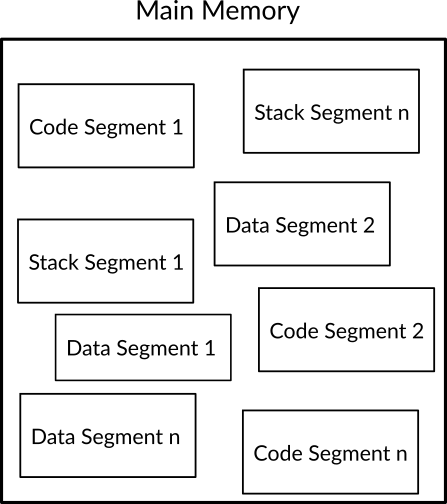
\includegraphics[width=0.35000\textwidth]{Figures/x86-ch/memory-segmented-view.png}
\caption{An Example of The Segmented View of the
Memory}\label{fig:memory_segmented_view}
\end{figure}

\subsection{Segmentation in Real Mode}\label{segmentation-in-real-mode}

For the sake of clarity, let's discuss the details of segmentation under
real mode first. We have said that logical views (of anything) should be
mapped to the physical view either by software or hardware, in this
case, the segmentation view is realized and mapped to the architecture
of the physical main memory by the x86 processor itself, that is, by the
hardware. So, we have a logical view, which is the concept of
segmentation which divides a program into separated segments, and the
actual physical main memory view which is supported by the real RAM
hardware and sees the data as a big array of bytes. Therefore, we need
some tools to implement (map) the logical view of segmentation on top
the actual hardware.

For this purpose, special registers named \emph{segment registers} are
presented in x86, the size of each segment register is \lstinline!16!
bits and they are: \lstinline!CS! which is used to define the code
segment. \lstinline!SS! which is used to define the stack segment.
\lstinline!DS!, \lstinline!ES!, \lstinline!FS! and \lstinline!GS! which
can be used to define data segments, that means each program can have up
to four data segments. Each segment register stores the \emph{starting
memory address} of a segment and here you can start to observe the
mapping between the logical and physical view. In real mode, the size of
each segment is \lstinline!64KB! and as we have said we can reach any
byte inside a segment by using the \emph{offset} of the required byte,
you can see the resemblance between a memory address of the basic view
of memory and an offset of the segmentation view of memory \footnote{The
  concept and term of offset is not exclusive to segmentation, it is
  used on other topics related to the memory.}.

Let's take an example to make the matter clear, assume that we have a
code of some program loaded into the memory and its starting physical
memory address is \lstinline!100d!, that is, the first instruction of
this program is stored in this address and the next instructions are
stored right after this memory address one after another. To reach the
first byte of this code we use the offset \lstinline!0!, so, the whole
physical address of the first byte will be \lstinline!100:0d!, as you
can see, the part before the colon is the starting memory address of the
code and the part after the colon is the offset that we would like to
reach and read the byte inside it. In the same way, let's assume we
would like to reach the offset \lstinline!33!, which means the byte
\lstinline!34! inside the loaded code, then the physical address that we
are trying to reach is actually \lstinline!100:33d!. To make the
processor handle this piece of code as the \emph{current} code segment
then its starting memory address should be loaded into the register
\lstinline!CS!, that is, setting the value \lstinline!100d! to
\lstinline!CS!, so, we can say in other words that \lstinline!CS!
contains the starting memory address of currently executing code segment
(for short: current code segment).

As we have said, the x86 processor always run with the mind that the
segmentation is in use. So, let's say it is executing the following
assembly instruction \lstinline!jmp 150d! which jumps to the address
\lstinline!150d!. What really happens here is that the processor
consider the value \lstinline!150d! as an offset instead of a full
memory address, so, what the instruction requests from the processor
here is to jump to the offset \lstinline!150! which is inside the
current code segment, therefore, the processor is going to retrieve the
value of the register \lstinline!CS! to know what is the starting memory
address of the currently active code segment and append the value
\lstinline!150! to it. Say, the value of \lstinline!CS! is
\lstinline!100!, then the memory address that the processor is going to
jump to is \lstinline!100:150d!.

This is also applicable on the internal work of the processor, do you
remember the register \lstinline!IP! which is the instruction pointer?
It actually stores the offset of the next instruction instead of the
whole memory address of the instruction. Any call (or jump) to a code
inside the same code segment of the caller is known as \emph{near call
(or jump)}, otherwise is it a \emph{far call (or jump)}. Again, let's
assume the current value of \lstinline!CS! is \lstinline!100d! and you
want to call a label which is on the memory location \lstinline!900:1d!,
in this situation you are calling a code that reside in a different code
segment, therefore, the processor is going to take the first part of the
address which is\lstinline!900d!, loads it to \lstinline!CS! then loads
the offset \lstinline!1d! in \lstinline!IP!. Because this call caused
the change of \lstinline!CS! value to another value, it is a far call.

The same is exactly applicable to the other two types of segments and of
course, the instructions deal with different segment types based on
their functionality, for example, you have seen that \lstinline!jmp! and
\lstinline!call! deal the code segment in \lstinline!CS!, that's because
of their functionality which is related to the code. Another example is
the instruction \lstinline!lodsb! which deals with the data segment
\lstinline!DS!, the instruction \lstinline!push! deals with the stack
segment \lstinline!SS! and so on.

\subsubsection{Segmentation Used in the
Bootloader}\label{segmentation-used-in-the-bootloader}

In the previous chapter, when we wrote the bootloader, we have dealt
with the segments. Let's get back to the source code of the bootloader,
you remember that the firmware loads the bootloader on the memory
location \lstinline!07C0h! and because of that we started our bootloader
with the following lines.

\begin{lstlisting}
    mov ax, 07C0h
    mov ds, ax
\end{lstlisting}

Here, we told the processor that the data segment of our program (the
bootloader) starts in the memory address \lstinline!07C0h! \footnote{Yes,
  all segments can be on the same memory location, that is, there is a
  \lstinline!64KB! segment of memory which is considered as the
  currently active code segment, data segment and stack segment. We have
  already mentioned that when we have discussed how to implement
  flat-memory model on x86.}, so, if we refer to the memory to read or
write \textbf{data}, the processor starts with the memory address
\lstinline!07C0h! which is stored in the data segment register
\lstinline!ds! and then it appends the offset that we are referring to,
in other words, any reference to data by the code being executed will
make the processor to use the value in data segment register as the
beginning of the data segment and the offset of referred data as the
rest of the address, after that, this physical memory address of the
referred data will be used to perform the instruction. An example of
instructions that deal with data in our bootloader is the line
\lstinline!mov si, title_string!.

Now assume that BIOS has set the value of \lstinline!ds! to
\lstinline!0! (it can be any other value) and jumped to our bootloader,
that means the data segment in the system now starts from the physical
memory address \lstinline!0! and ends at the physical memory address
\lstinline!65535! since the maximum size of a segment in real-mode is
64KB. Now let's take the label \lstinline!title_string! as an example
and let's assume that its offset in the binary file of our bootloader is
\lstinline!490!, when the processor starts to execute the line
\lstinline!mov si, title_string! \footnote{Which loads the physical
  memory address of \lstinline!title_string! to the register
  \lstinline!si!.} it will, somehow, figures that the offset of
\lstinline!title_string! is \lstinline!490! and based on the way that
x86 handles memory accesses the processor is going to think that we are
referring to the physical memory address \lstinline!490! since the value
of \lstinline!ds! is \lstinline!0!, but in reality, the correct physical
memory address of \lstinline!title_string! is the offset \lstinline!490!
\textbf{inside} the memory address \lstinline!07C0h! since our
bootloader is loaded into this address and not the physical memory
address \lstinline!0!, so, to be able to reach to the correct addresses
of the data that we have defined in our bootloader and that are loaded
with the bootloader starting from the memory address \lstinline!07C0h!
we need to tell the processor that our data segment starts from
\lstinline!07C0h! and with any reference to data, it should calculate
the offset of that data starting from this physical address, and that
exactly what these two lines do, in other words, change the current data
segment to another one which starts from the first place of our
bootloader.

The second use of the segments in the bootloader is when we tried to
load the kernel from the disk by using the BIOS service
\lstinline!13h:02h! in the following code.

\begin{lstlisting}
    mov ax, 0900h
    mov es, ax
    
    mov ah, 02h
    mov al, 01h
    mov ch, 0h
    mov cl, 02h
    mov dh, 0h
    mov dl, 80h
    mov bx, 0h
    int 13h
\end{lstlisting}

You can see here, we have used the other data segment \lstinline!ES! to
define a new data segment that starts from the memory address
\lstinline!0900h!, we did that because the BIOS service
\lstinline!13h:02h! loads the required content (in our case the kernel)
to the memory address \lstinline!ES:BX!, for that, we have defined the
new data segment and set the value of \lstinline!bx! to \lstinline!0h!.
That means the code of the kernel will be loaded on
\lstinline!0900:0000h! and because of that, after loading the kernel
successfully we have performed a far jump.

\begin{lstlisting}
jmp 0900h:0000
\end{lstlisting}

Once this instruction is executed, the value of \lstinline!CS! will be
changed from the value \lstinline!07C0h!, where the bootloader resides,
to the value \lstinline!0900h! where the kernel resides and the value of
\lstinline!IP! register will be \lstinline!0000! then the execution of
the kernel is going to start.

\subsection{Segmentation in Protected
Mode}\label{segmentation-in-protected-mode}

The fundamentals of segmentation in protected mode is exactly same as
the ones explained in real mode, but it has been extended to provide
more features such as \emph{memory protection}. In protected mode, a
table named \emph{global descriptor table} (\lstinline!GDT!) is
presented, this table is stored in the main memory and its starting
memory address is stored in the special purpose register
\lstinline!GDTR! as a reference, each entry in this table called a
\emph{segment descriptor} which has the size \lstinline!8! bytes and
they can be referred to by an index number called \emph{segment
selector} \footnote{This is a \textbf{relaxed} definition of segment
  selector, a more accurate one will be presented later.} which is the
offset of the entry inside \lstinline!GDT! table, For example, the
offset of the first entry in \lstinline!GDT! is \lstinline!0!, and
adding this offset with the value of \lstinline!GDTR! gives us the
memory address of that entry, however, the first entry of
\lstinline!GDT! should not be used by the operating system.

An entry of \lstinline!GDT! (a segment descriptor), defines a segment
(of any type) and has the information that is required by the processor
to deal with that segment. The starting memory address of the segment is
stored in its descriptor \footnote{In real mode, the starting address of
  the segment is stored directly on the corresponding segment register
  (e.g. \lstinline!CS! for code segment).}, also, the size (or limit) of
the segment. The segment selector of the currently active segment should
be stored in the corresponding segment register.

To clarify the matter, consider the following example. Let's assume we
are currently running two programs and their code are loaded into the
main memory and we would like to separate these two pieces of code into
a couple of code segments. The memory area \lstinline!A! contains code
of the first program and starts from the memory address \lstinline!800!
while the memory area \lstinline!B! contains the code of the second
program\lstinline!B! and starts in the memory address \lstinline!900!.
Assume that the starting memory address of \lstinline!GDT! is
\lstinline!500! which is already loaded in \lstinline!GDTR!.

To make the processor consider \lstinline!A! and \lstinline!B! as code
segments we should define a segment descriptor for each one of them. We
already know that the size of a segment descriptor is \lstinline!8!
bytes, so, if we define a segment descriptor for the segment
\lstinline!A! as entry \lstinline!1! (remember that the entries on
\lstinline!GDT! starts from zero) then its offset (segment selector) in
\lstinline!GDT! will be \lstinline!8! (\lstinline!1 * 8!), the segment
descriptor of \lstinline!A! should contain the starting address of
\lstinline!A! which is \lstinline!800!, and we will define the segment
descriptor of \lstinline!B! as entry \lstinline!2! which means its
offset (segment selector) will be \lstinline!16! (\lstinline!2 * 8!).

Let's assume now that we want the processor to execute the code of
segment \lstinline!A!, we already know that the processor consults the
register \lstinline!CS! to decide which code segment is currently active
and should be executed next, for that, the \textbf{segment selector} of
code segment \lstinline!A! should be loaded in \lstinline!CS!, so the
processor can start executing it. In real mode, the value of
\lstinline!CS! and all other segment registers was a memory address, on
the other hand, in protected mode, the value of \lstinline!CS! and all
other segment registers is a segment selector.

In our situation, the processor takes the segment selector of
\lstinline!A! from \lstinline!CS! which is \lstinline!8! and starting
from the memory address which is stored in \lstinline!GDTR! it walks
\lstinline!8! bytes, so, if \lstinline!GDTR = 500!, the processor will
find the segment descriptor of \lstinline!A! in the memory address
\lstinline!508!. The starting address of \lstinline!A! will be found in
its segment descriptor and the processor can use it with the value of
register \lstinline!EIP! to execute \lstinline!A!'s code. Let's assume a
far jump is occurred from \lstinline!A! to \lstinline!B!, then the value
of \lstinline!CS! will be changed to the segment selector of
\lstinline!B! which is \lstinline!16!.

\subsubsection{The Structure of Segment
Descriptor}\label{the-structure-of-segment-descriptor}

A segment descriptor is an \lstinline!8! bytes entry of global
descriptor table which stores multiple \emph{fields} and \emph{flags}
that describe the properties of a specific segment in the memory. With
each memory reference to any segment, the processor is going to consult
the descriptor that describes the segment in question to obtain basic
information like starting memory address of this segment.

Beside the basic information, a segment descriptor stores information
the helps in memory protection, due to that, segmentation in x86
protected-mode is considered as a way for memory protection and not a
mere logical view of the memory, so each memory reference is being
monitored by the processor.

By using those properties that are related to memory protection, the
processor will be able to protect the different segments on the system
from each other and not letting some less privileged to call a code or
manipulate data which belong to more privileged area of the system, a
concrete example of that is when a userspace software (e.g.~Web Browser)
tries to modify an internal data structure in the kernel.

In the following subsections, each field and flag of segment descriptor
will be explained, but before getting started we need to note that in
here and in Intel's official x86 manual the term \emph{field} is used
when the size of the value that should be stored in the descriptor is
\textbf{more than} \lstinline!1! bit, for example the segment's starting
memory address is stored in \lstinline!4! bytes, then the place where
this address is stored in the descriptor is called a field, otherwise
when the term \emph{flag} is used that means the size of the value is
\lstinline!1! bit.

\paragraph{Segment's Base Address and
Limit}\label{segments-base-address-and-limit}

The most important information about a segment is its starting memory
address, which is called the \emph{base address} of a segment. In real
mode, the base address was stored in the corresponding segment register
directly, but in protected mode, where we have more information about a
segment than mere base address, this information is stored in the
descriptor of the segment \footnote{Reminder: In protected mode, the
  corresponding segment register stores the selector of the currently
  active segment.}.

When the currently running code refers to a memory address to read from
it, write to it (in the case of data segments) or call it (in the case
of code segments) it is actually referring to a specific segment in the
system \footnote{And it \textbf{should}, since segmentation is enabled
  by default in x86 and cannot be disabled.}. For the simplicity of next
discussions, we call this memory address, which is referenced by the
currently running code, the \emph{generated memory address} because, you
know, it is generated by the code.

Any generated memory address in x86 architecture is not an actual
physical memory address \footnote{Remember our discussion of the
  difference between our logical view of the memory (e.g.~segmentation)
  and the actual physical hardware}, that means, if you hypothetically
get a generated memory address and try to get the content of its
physical memory location, the obtained data will not be same as the data
which is required by the code. Instead, a generated memory address is
named by Intel's official manual a \emph{logical memory address}
because, you know, it is not real memory address, \textbf{it is}
logical. Every logical memory address refers to some byte in a specific
segment in the system, and to be able to obtain the data from the actual
physical memory, this logical memory address should be \emph{translated}
to a \emph{physical memory address} \footnote{We can see here how
  obvious the mapping between the logical view of the memory and the
  real-world memory.}.

The logical memory address in x86 may pass \textbf{two} translation
processes instead of one in order to obtain the physical memory address.
The first address translation is performed on a logical memory address
to obtain a \emph{linear memory address} which is another not real and
not physical memory address which is there in x86 architecture because
of paging feature. If paging \footnote{Don't worry about paging right
  now. It will be discussed later in this book. All you need to know now
  is that paging is another logical view of the memory. Paging is
  disabled by default in x86 which makes it an optional feature unlike
  segmentation.} is enabled in the system, a second translation process
takes place on this linear memory address to obtain the real physical
memory address. If paging is disabled, the linear memory address which
is generated by the first translation process is same as the physical
memory address. We can say that the first translation is there in x86
due to the segmentation view of memory, while the second translation is
there in x86 due to the paging view of memory.

\begin{figure}
\centering
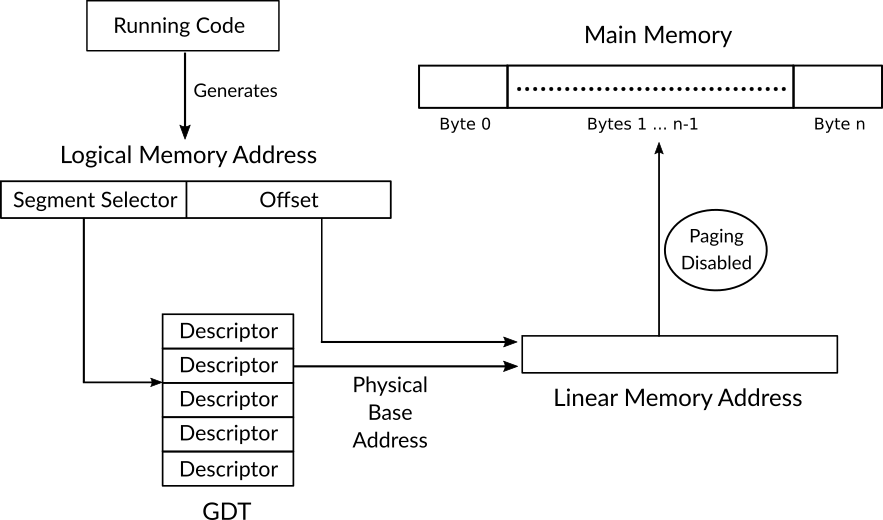
\includegraphics[width=0.90000\textwidth]{Figures/x86-ch/logical-memory-address-translation.png}
\caption{Shows How a Logical Memory Address is Translated to a Linear
Memory Address (Which Represents a Physical Address when Paging is
Disabled).}\label{fig:logical_memory_address_translation}
\end{figure}

For now, our focus will be on the translation from a logical memory
address to a linear memory address which is same as the physical memory
address since paging feature is disabled by default in x86. Each logical
memory address consists of two parts, a \lstinline!16! bits segment
selector and a \lstinline!32! bits offset. When the currently running
code generates a logical memory address (for instance, to read some data
from memory) the processor needs to perform the translation process to
obtain the physical memory address as the following. First, it reads the
value of the register \lstinline!GDTR! which contains the starting
physical memory address of \lstinline!GDT!, then it uses the
\lstinline!16-bit! segment selector in the generated logical address to
locate the descriptor of the segment that the code would like to read
the data from, inside segment's descriptor, the physical base address
(the starting physical address) of the requested segment can be found,
the processor obtains this base address and adds the \lstinline!32-bit!
offset from the logical memory address to the base address to obtain the
last result, which is the linear memory address.

During this operation, the processor uses the other information in the
segment descriptor to enforce the policies of memory protection. One of
these policies is defined by the \emph{limit} of a segment which
specifies its size, if the generated code refers to an offset which
exceeds the limit of the segment, the processor should stop this
operation. For example, assume hypothetically that the running code has
the privilege to read data from data segment \lstinline!A! and in the
physical memory another data segment \lstinline!B! is defined right
after the limit of \lstinline!A!, which means if we can exceed the limit
of \lstinline!A! we will able to access the data inside \lstinline!B!
which is a critical data segment that stores kernel's internal data
structures and we don't want any code to read from it or write to it in
case this code is not privileged to do so. This can be achieved by
specifying the limit of \lstinline!A! correctly, and when the
unprivileged code tries maliciously to read from \lstinline!B! by
generating a logical memory address that has an offset which exceeds the
limit of \lstinline!A! the processor prevents the operation and protects
the content of segment \lstinline!B!.

The limit, or in other words, the size of a given segment is stored in
the \lstinline!20! bits \emph{segment limit field} of that segment
descriptor and how the processor interprets the value of segment limit
field depends on the \emph{granularity flag} (G flag) which is also
stored in the segment's descriptor, when the value of this flag is
\lstinline!0! then the value of the limit field is interpreted as bytes,
let's assume that the limit of a given segment is \lstinline!10! and the
value of granularity flag is \lstinline!0!, that means the size of this
segment is \lstinline!10! \textbf{bytes}. On the other hand, when the
value of granularity flag is \lstinline!1!, the value of segment limit
field will be interpreted as of \lstinline!4KB! units, for example,
assume in this case that the value of limit field is also \lstinline!10!
but G flag = \lstinline!1!, that means the size of the segment will be
\lstinline!10! of \lstinline!4KB! units, that is, \lstinline!10 * 4KB!
which gives us \lstinline!40KB! which equals \lstinline!40960! bytes.

Because the size of segment limit field is \lstinline!20! bits, that
means the maximum numeric value it can represent is
\lstinline!2^20 = 1,048,576!, which means if G flag equals \lstinline!0!
then the maximum size of a specific segment can be \lstinline!1,048,576!
\textbf{bytes} which equals \lstinline!1MB!, and if G flag equals
\lstinline!1! then the maximum size of a specific segment can be
\lstinline!1,048,576! of \lstinline!4KB! units which equals
\lstinline!4! \textbf{GB}.

Getting back to the structure of descriptor, the bytes \lstinline!2!,
\lstinline!3! and \lstinline!4! of the descriptor store the \emph{least
significant bytes} of segment's base address and the byte \lstinline!7!
of the descriptor stores the \emph{most significant byte} of the base
address, the total is \lstinline!32! bits for the base address. The
bytes \lstinline!0! and \lstinline!1! of the descriptor store the
\emph{least significant bytes} of segment's limit and byte \lstinline!6!
stores the \emph{most significant byte} of the limit. The granularity
flag is stored in the most significant \textbf{bit} of the the byte
\lstinline!6! of the descriptor.

Before finishing this subsection, we need to define the meaning of
\emph{least significant} and \emph{most significant} byte or bit. Take
for example the following binary sequence which may represent anything,
from a memory address value to a \lstinline!UTF-32! character.

\textbf{0}111 0101 0000 0000 0000 0000 0100 110\emph{1}

You can see the first bit from left is on bold format and its value is
\lstinline!0!, based on its position in the sequence we call this bit
the \emph{most significant bit} or \emph{high-order bit}, while the last
bit on the right which is in italic format and its value is
\lstinline!1! is known as \emph{least significant bit} or
\emph{low-order bit}. The same terms can be used on byte level, given
the same sequence with different formatting.

\textbf{0111 0101} 0000 0000 0000 0000 \emph{0100 1101}

The first byte (\lstinline!8! bits) on the left which is in bold format
and its value is \lstinline!0111 0101! is known as \emph{most
significant byte} or \emph{high-order byte} while the last byte on the
right which is on italic format and its value is \lstinline!0100 1101!
is known as \emph{least significant byte} or \emph{low-order byte}.

Now, imagine that this binary sequence is the base address of a segment,
then the least significant \lstinline!3! bytes of it will be stored in
bytes \lstinline!2!, \lstinline!3! and \lstinline!4! of the descriptor,
that is, the following binary sequence.

\begin{lstlisting}
0000 0000 0000 0000 0100 1101
\end{lstlisting}

While the most significant byte of the binary sequence will be stored in
the \lstinline!7th! byte of the descriptor, that is, the following
binary sequence.

\begin{lstlisting}
0111 0101
\end{lstlisting}

\paragraph{Segment's Type}\label{segments-type}

Given any binary sequence, it doesn't have any meaning until some
context is added. For example, what does the binary sequence
\lstinline!1100 1111 0000 1010! represents? It could represent anything,
a number, characters, pixels on an image or even all of them based on
how its user interprets it. When an agent (e.g.~a bunch of code in
running software or the processor) works with a binary sequence, it
should know what does this binary sequence represent to be able to
perform useful tasks. In the same manner, when a segment is defined, the
processor (the agent) should be told how to interpret the content inside
this segment, that is, the type of the segment should be known by the
processor.

Till this point, you probably noticed that there is at least two types
of segments, code segment and data segment. The content of the former
should be machine code that can be executed by the processor to perform
some tasks, while the content of the latter should be data (e.g.~values
of constants) that can be used by a running code. These two types of
segments (code and data) belong to the category of \emph{application
segments}, there is another category of segment types which is the
category of \emph{system segments} and it has many different segment
types belong to it.

Whether a specific segment is an application or system segment, this
should be mentioned in the descriptor of the segment in a flag called
\emph{S flag} or \emph{descriptor type flag} which is the fifth
\textbf{bit} in \textbf{byte} number \lstinline!5! of the segment
descriptor. When the value of S flag is \lstinline!0!, then the segment
is considered as a system segment, while it is considered as an
application segment when the value of S flag is \lstinline!1!. Our
current focus is on the latter case.

As we have mentioned before, an application segment can be either code
or data segment. Let's assume some application segment has been
referenced by a currently running code, the processor is going to
consult the descriptor of this segment, and by reading the value of S
flag (which should be \lstinline!1!) it will know that the segment in
question is an application segment, but which of the two types? Is it a
code segment or data segment? To answer this question for the processor,
this information should be stored in a field called \emph{type field} in
the segment's descriptor.

Type field in segment descriptor is the first \lstinline!4! bits
(nibble) of the fifth byte and the most significant bit specifies if the
application segment is a code segment (when the value of the bit is
\lstinline!1!) or a data segment (when the value of the bit is
\lstinline!0!). Doesn't matter if the segment is a code or data segment,
in the both cases the least significant bit of type field indicates if
the segment is \emph{accessed} or not, when the value of this flag is
\lstinline!1!, that means the segment has been written to or read from
(AKA: accessed), but if the value of this flag is \lstinline!0!, that
means the segment has not been accessed. The value of this flag is
manipulated by the processor in one situation only, and that's happen
when the selector of the segment in question is loaded into a segment
register. In any other situation, it is up to the operating system to
decide the value of accessed flag. According to Intel's manual, this
flag can be used for virtual memory management and for debugging.

\subparagraph{Code Segment Flags}\label{code-segment-flags}

When the segment is a code segment, the second most significant bit
(tenth bit) is called \emph{conforming flag} (also called \lstinline!C!
flag) while the third most significant bit (ninth bit) called
\emph{read-enabled flag} (also called \lstinline!R! flag.). Let's start
our discussion with the simplest among those two flags which is the
read-enabled flag. The value of this flag indicates how the code inside
the segment in question can be used, when the value of read-enabled flag
is \lstinline!1! \footnote{Which means \textbf{do} enable read, since
  \lstinline!1! is equivalent to \lstinline!true! in the context of
  flags.}, that means the content of the code segment can be executed
\textbf{and} read from, but when the value of this flag is \lstinline!0!
\footnote{Which means \textbf{don't} enable read.} that means the
content of the code segment can be \textbf{only} executed and cannot
read from. The former option can be useful when the code contains data
inside it (e.g.~constants) and we would like to provide the ability of
reading this data. When read is enabled for the segment in question, the
selector of this segment can also be loaded into one of data segment
registers \footnote{Which makes sense, enabling reads from a code
  segment means it contains data also.}.

The conforming flag is related to the privilege levels that we had an
overview about them previously in this chapter. When a segment is
conforming, in other words, the value of conforming flag is
\lstinline!1!, that means a code which runs in a less-privileged level
can call this segment which runs in a higher privileged level while
keeping the current privilege level of the environment same as the one
of the caller instead of the callee.

For example, let's assume for some reason a kernel's designer decided to
provide simple arithmetic operations (such as addition and subtraction)
for user applications from the kernel code, that is, there is no other
way to perform these operations in that system but this code which is
provided by the kernel. As we know, kernel's code should run in
privilege level \lstinline!0! which is the most-privileged level, and
let's assume a user application which runs in privilege level
\lstinline!3!, a less-privileged level, needs to perform an addition
operation, in this case a kernel code, which should be protected by
default from being called by less-privileged code, should be called to
perform the task, this can only realized if the code of addition
operation is provided as a conforming segment, otherwise the processor
is going to stop this action where a less-privileged code calls a
more-privileged code.

Also you should note that the code of addition operation is going to run
in privilege level \lstinline!3! although it is a part of the kernel
which runs in privilege level \lstinline!0! and that's because of the
original caller which runs in the privilege level \lstinline!3!.
Furthermore, although conforming segment can be called by a
less-privilege code (e.g.~user application calls the kernel), the
opposite cannot be done (e.g.~the kernel calls a user application's
code) and the processor is going to stop the operation.

\subparagraph{Data Segment Flags}\label{data-segment-flags}

When the segment is data segment, the second most significant bit (tenth
bit) is called expansion-direction flag (also called \lstinline!E! flag)
while the third most significant bit (ninth bit) is called write-enabled
flag (also called \lstinline!W! flag). The latter one gives us the
ability to make some data segment a read-only when its value is
\lstinline!0!, or we can make a data segment both \textbf{writable} and
readable by setting the value of write-enabled flag to \lstinline!1!.

While the expansion-direction flag and its need will be examined in
details when we discuss x86 run-time stack in this chapter, what we need
to know right now is that when the value of this flag is \lstinline!0!,
the data segment is going to expand \textbf{up} (in Intel's terms), but
when the value of this flag is \lstinline!1!, the data segment is going
to expand \textbf{down} (in Intel's terms).

A last note about data segments is that all of them are
\textbf{non-conforming}, that is, a less-privileged code cannot access a
data segment in a more-privileged level. Furthermore, all data segments
can be accessed by a more-privileged code.

\paragraph{Segment's Privilege Level}\label{segments-privilege-level}

In our previous discussions, we have stated that a specific segment
should belong to a privilege level and based on this privilege level the
processor decides the protection properties of the segment in question,
for example, whether that segment is a kernel-mode or user-mode segment
and which privilege level a running code should belong to in order to be
able to reach to this segment

A field called \emph{descriptor privilege level} (DPL) in segment
descriptor is where the operating system should set the privilege level
of a given segment. The possible values of this field, as we know, are
\lstinline!0!, \lstinline!1!, \lstinline!2! and \lstinline!3!, we have
already discussed the meanings of these values previously in this
chapter. Descriptor privilege level field occupies the second and third
most significant bits of byte \lstinline!5! in a descriptor.

\paragraph{Segment's Present}\label{segments-present}

One of common operations that is performed in a running system is
loading data from secondary storage (e.g.~hard disk) into the memory and
one example of that is loading a program code into the memory when the
user of the system request to run an instance of a program, so, creating
a new segment descriptor (hence, creating new segment in the memory) for
this data may precede the completion of loading the data into the main
memory, therefore, there could be some segment descriptors in the system
that points to memory locations that don't contain the real data yet.

In this case, we should tell the processor that the data in the memory
location that a specific descriptor points to is not the real data, and
the real segment is not presented in the memory yet, this helps the
processor to generate error when some code tries to access \footnote{We
  use the term \emph{access} here for both types of application
  segments. While this term is valid for data segment, we mean
  \emph{execute} for code segment.} the segment's data. To tell the
processor whether a segment is presented in the memory or not,
\emph{segment-present flag} (P flag) can be used, when its value is
\lstinline!1! that means the segment is present in memory, while the
value \lstinline!0! means the segment is not present in memory, this
flag is the most significant bit of byte \lstinline!5! of a descriptor.

\paragraph{Other Flags}\label{other-flags}

We have covered all segment's descriptor fields and flags but three
flags. The name of the first one changes depending on the type of the
segment and it occupies the second most significant bit in the byte
\lstinline!6!. When the segment in question is a code segment, this flag
is called \emph{default operation size} (D flag). When the processor
executes the instructions it uses this flag to decide the length of the
operands, depending on the currently executing instruction, if the value
of D flag is \lstinline!1! the processor is going to assume the operand
has the size of \lstinline!32! bits if it is a memory address, and
\lstinline!32! bits or \lstinline!8! bits if it is not a memory address.
If the value of D flag is \lstinline!0! the processor is going to assume
the operand has the size of \lstinline!16! bits if it is a memory
address, and \lstinline!16! bits or \lstinline!8! bits operand if it is
not a memory address.

When the segment in question is a stack segment \footnote{The processor
  knows it is a stack segment if the segment selector is loaded into
  stack segment selector register \lstinline!SS!}, the same flag is
called \emph{default stack pointer size} (B flag), and it decides the
size of the memory address (as a value) which points to the stack, this
memory address is known as \emph{stack pointer} and it is being used
implicitly by stack instructions such as \lstinline!push! and
\lstinline!pop!. When the value of B flag is \lstinline!1!, then the
size of stack pointer will be \lstinline!32! bits and its value will be
stored in the register \lstinline!ESP! (rather then \lstinline!SP!),
When the value of B flag is \lstinline!0!, then the size of stack
pointer will be \lstinline!16! bits and its value will be stored in the
register \lstinline!SP! (rather then \lstinline!ESP!).

When the segment in question is a data segment that grows upward, this
flag is called \emph{upper bound flag} (B flag), when its value is
\lstinline!1! the maximum possible size of the segment will be
\lstinline!4GB!, otherwise, the maximum possible size of the segment
will be \lstinline!64KB!. Anyway, the value of this flag (D/B flag)
\textbf{should} be \lstinline!1! for \lstinline!32-bit! code and data
segments (stack segments are included of course) and it should be
\lstinline!0! for \lstinline!16-bit! code and data segments.

The second flag is known as \emph{64-bit code segment flag} (L flag)
which is the third most significant bit in the byte \lstinline!6! and
from its name we can tell that this flag is related to code segments. If
the value of this flag is \lstinline!1! that means the code inside the
segment in question is a \lstinline!64-bit! code while the value
\lstinline!0! means otherwise \footnote{In terms of Intel's manual:
  \emph{compatibility mode}.}. When we set the value of L flag to
\lstinline!1! the value of D/B flag should be \lstinline!0!.

The final flag is the fourth most significant bit in the byte
\lstinline!6!, the value of this flag has no meaning for the processor,
hence, it will not use it to make any decisions upon the segment in the
question as we have seen on all other flags and fields. On the other
hand, this flag is available for the operating system to use it in
whatever way it needs, or just ignores it by set it to any of possible
values ,\lstinline!0! or \lstinline!1! since it is one bit.

\subsubsection{\texorpdfstring{The Special Register
\texttt{GDTR}}{The Special Register GDTR}}\label{the-special-register-gdtr}

The special register \lstinline!GDTR! stores the base physical address
\footnote{More accurately, the linear address. Refer to discussion of
  memory translation process in this chapter.} of the global descriptor
table, that is, the starting point of \lstinline!GDT! table. Also, the
same register stores the limit (or size) of the table.

\begin{figure}
\centering
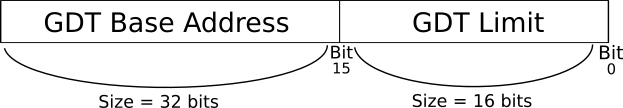
\includegraphics[width=0.50000\textwidth]{Figures/x86-ch/Fig16062021_0.png}
\caption{GDTR Structure}\label{fig:16062021_0}
\end{figure}

To load a value into the register \lstinline!GDTR! the x86 instruction
\lstinline!lgdt!, which stands for \emph{load} global descriptor table,
should be used. This instruction takes one operand which is the whole
value that should be loaded into \lstinline!GDTR!, the structure of this
value should be similar to the structure of \lstinline!GDTR! itself
which is shown in figure \ref{fig:16062021_0}. The figure shows that the
total size of \lstinline!GDTR! is \lstinline!48! bits divided into two
parts. The first part starts from bit \lstinline!0! (the least
significant bit) to bit \lstinline!15!, this part contains the limit of
\lstinline!GDT! table that we would like to load. The size of this part
of \lstinline!GDTR! register is \lstinline!16! bits which can represent
the value \lstinline!65,536! at maximum, that means the maximum size of
\lstinline!GDT! table can be \lstinline!64KB = 65,536 Bytes / 1024!, and
as we know, the size of each of descriptor is \lstinline!8! bytes, that
means the \lstinline!GDT! table can hold \lstinline!8,192! descriptors
at most. The second part of \lstinline!GDTR! starts from bit
\lstinline!16! to bit \lstinline!47! (the most significant bit) and
stores the base memory address of \lstinline!GDT! table that we would
like to load.

\subsubsection{Local Descriptor Table}\label{local-descriptor-table}

The global descriptor table is a system-wide table, in other words, it
is available for every process of the system. In addition to
\lstinline!GDT!, x86 provides us with ability to define \emph{local
descriptor tables} (\lstinline!LDT!) in protected-mode which have the
same functionality and structure of \lstinline!GDT!.

In contrary to \lstinline!GDT! table, multiple \lstinline!LDT! can be
defined in the system, and each one of them can be private to a specific
process that is currently running on the system, also, multiple running
processes can share a single \lstinline!LDT! that is considered private
for them by the kernel and no other processes can reach this given
\lstinline!LDT!. Anyway, how to use \lstinline!LDT! depends on how the
kernel is designed, and while \lstinline!GDT! is required in x86
architecture by default, \lstinline!LDT! on the other hand is optional
and the designer of the kernel is the one who is responsible to decide
whether to use \lstinline!LDT! or not.

Let's assume that we need to create a new \lstinline!LDT! table for
process \lstinline!A! which is currently running on the system, this
\lstinline!LDT! table is already filled with the descriptors that
describe the segments which belong to process \lstinline!A!. The
structure of the descriptors in \lstinline!LDT! is exactly same as the
one that we already described in this chapter. To tell the processor
that a given region of a memory is an \lstinline!LDT! table, a new
segment descriptor should be created in \lstinline!GDT!.

In our previous discussion of \lstinline!S! flag we mentioned that this
flag tells the processor whether a defined segment is an application
segment (S flag = \lstinline!1!) or a system segment (S flag =
\lstinline!0!), the segment of the memory that contains an
\lstinline!LDT! table is considered as a system segment, that is, the
value of \lstinline!S! flag in the descriptor that describes an
\lstinline!LDT! table should be \lstinline!0! and because there are
other types of system segments than \lstinline!LDT! then we should tell
the processor this system segment is an \lstinline!LDT! table, to do
that we should use the type field of the descriptor that we already
mentioned, the value of this field should be \lstinline!0010b!
(\lstinline!2d!) for descriptors that describe an \lstinline!LDT! table,
how the processor can tell which table should currently used for a given
segment \lstinline!GDT! or \lstinline!LDT! will be discussed in the next
subsection.

The x86 instruction \lstinline!lldt! is used to load the \lstinline!LDT!
table that we would like to use now into a special register named
\lstinline!LDTR! which is a \lstinline!16-bit! register that should
contain the segment selector \footnote{More accurate definition of a
  segment selector and its structure in protected-mode is presented in
  the next subsection.} in \lstinline!GDT! of the \lstinline!LDT! table
that we would like to use, in other words, the index of segment
descriptor which describe the \lstinline!LDT! table and which reside in
\lstinline!GDT! as an entry should be loaded into \lstinline!LDTR!
register.

\subsubsection{Segment Selector}\label{segment-selector}

As we know, the index (offset) of the descriptor that the currently
running code needs to use, whether this descriptor defines and code or
data segment, should be loaded into one of segment registers, but how
the can the processor tell if this index which is loaded into a segment
register is an index in the \lstinline!GDT! or \lstinline!LDT!?

\begin{figure}
\centering
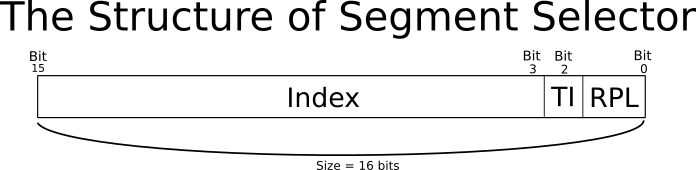
\includegraphics[width=0.50000\textwidth]{Figures/x86-ch/Fig17062021_0.png}
\caption{Segment Selector Structure}\label{fig:17062021_0}
\end{figure}

When we discussed segment selectors previously in this chapter we have
said that our definition of this concept is a \textbf{relaxed}
definition, that is, a simplified one that omits some details. In
reality, the index of a segment descriptor is just one part of a segment
selector, figure \ref{fig:17062021_0} shows the structure of a segment
selector, which is same as the structure of all segment registers
\lstinline!CS!, \lstinline!SS!, \lstinline!DS!, \lstinline!ES!,
\lstinline!FS! and \lstinline!GS!. We can see from the figure that the
size of a segment selector is \lstinline!16! bits and starting from the
least significant bit (bit \lstinline!0!), the first two bits
\lstinline!0! and \lstinline!1! are occupied by field known as
\emph{requester privilege level} (\lstinline!RPL!). Bit \lstinline!2! is
occupied by a flag named \emph{table indicator} (\lstinline!TI!), and
finally, the index of a segment descriptor occupies the field from bit
\lstinline!3! until bit \lstinline!15! of the segment selector. The
index field (descriptor offset) is already well-explained in this
chapter, so we don't need to repeat its details.

The table indicator flag (\lstinline!TI!) is the one which is used by
the processor to tell if the index in the segment selector is an index
in \lstinline!GDT!, when the value of \lstinline!TI! is \lstinline!0!,
or \lstinline!LDT!, when the value is \lstinline!1!. When the case is
the latter, the processor consults the register \lstinline!LDTR! to know
the index of the descriptor that defines the current \lstinline!LDT! in
the \lstinline!GDT! and by using this index, the descriptor of
\lstinline!LDT! is read from \lstinline!GDT! by the processor to fetch
the base memory address of the current \lstinline!LDT!, after that, the
index in the segment selector register can be used to get the required
segment descriptor from the current \lstinline!LDT! by using the latter
base memory address that just been fetched, of course these values are
cached by the processor for quick future access.

In our previous discussions of privilege levels we have discussed two
values, current privilege level (\lstinline!CPL!) which is the privilege
level of the currently executing code and descriptor privilege level
(\lstinline!DPL!) which is the privilege level of a given segment, the
third value which contributes to the privilege level checks in x86 is
\emph{requester privilege level} (\lstinline!RPL!) which is stored in
the segment selector, necessarily, \lstinline!RPL! has four possible
values \lstinline!0!, \lstinline!1!, \lstinline!2! and \lstinline!3!.

To understand the role of \lstinline!RPL! let's assume that a process
\lstinline!X! is running in a user-mode, that is, in privilege level
\lstinline!3!, this process is a malicious process that aims to gain an
access to some important kernel's data structure, at some point of time
the process \lstinline!X! calls a code in the kernel and passes the
segment selector of the more-privileged data segment to it as a
parameter, the kernel code runs in the most privileged level and can
access all privileged data segment by simply loading the required data
segment selector to the corresponding segment register, in this case the
\lstinline!RPL! is set to \lstinline!0! maliciously by process
\lstinline!X!, since the kernel runs on the privilege level
\lstinline!0! and \lstinline!RPL! is \lstinline!0!, the required segment
selector by process \lstinline!X! will be loaded and the malicious
process \lstinline!X! will be able to gain access to the data segment
that has the sensitive data.

To solve this problem, \lstinline!RPL! should be set to the
\textbf{requester} privilege level by the kernel to load the required
data segment, in our example, the requester (the caller) is the process
\lstinline!X! and its privilege level is \lstinline!3! and the current
privilege level is \lstinline!0! since the kernel is running, but
because the caller has a less-privileged level the kernel should set the
\lstinline!RPL! of the required data segment selector to \lstinline!3!
instead of \lstinline!0!, this tells the processor that while the
currently running code in a privilege level \lstinline!0! the code that
called it was running in privilege level \lstinline!3!, so, any attempt
to reach a segment which its selectors \lstinline!RPL! is larger than
\lstinline!CPL! should be denied, in other words, the kernel should not
reach privileged segments in behalf of process \lstinline!X!. The x86
instruction \lstinline!arpl! can be used by the kernel's code to change
the \lstinline!RPL! of the segment selector that has been requested by
less-privileged code to access to the privilege level of the caller, as
in the example of process \lstinline!X!.

\section{x86 Run-time Stack}\label{x86-run-time-stack}

A user application starts its life as a file stored in user's hard disk,
at this stage it does nothing, it is just a bunch of binary numbers that
represent the machine code of this application, when the user decides to
use this application and opens it, the operating system loads this
application into the memory and in this stage this user application
becomes a process, we mentioned before that the term ``process'' is used
in operating systems literature to describe a running program, another
well-known term is \emph{task} which is used by Linux kernel and has the
same meaning.

Typically, the memory of a process is divided into multiple regions and
each one of them stores a different kind of application's data, one of
those regions stores the machine code of the application in the memory,
there are also two important regions of process' memory, the first one
is known as \emph{run-time heap} (or just \textbf{heap} for short) which
provides an area for dynamically allocated objects (e.g.~variables), the
second one is known as \emph{run-time stack} (or \textbf{stack} for
short), it's also known as \emph{call stack} but we are going to stick
to the term run-time stack in our discussions. Please note that the
short names of run-time stack (that is, stack) and run-time heap (that
is, heap) are also names for \textbf{data structures}. As we will see
shortly, a data structure describes a way of storing data and how to
manipulate this data, while in our current context these two terms are
used to represent \textbf{memory regions} of a running process although
the stack (as memory region) uses stack data structure to store the
data. Due to that, here we use the more accurate term \emph{run-time
stack} to refer the memory region and \emph{stack} to refer the data
structure.

Run-time stack is used to store the values of local variables and
function parameters, we can say that the run-time stack is a way to
implement \emph{function's invocation} which describes how function
\lstinline!A! can call function \lstinline!B!, pass to it some
parameters, return back to the same point of code where function
\lstinline!A! called function \lstinline!B! and finally get the returned
value from function \lstinline!B!, the implementation details of these
steps is known as \emph{calling convention} and the run-time stack is
one way of realizing these steps. There are multiple known calling
conventions for x86, different compilers and operating systems may
implement different calling conventions, we are not going to cover those
different methods but what we need to know that, as we said, those
different calling conventions use the run-time stack as a tool to
realize function's invocation. The memory region in x86 which is called
run-time stack uses a data structure called \emph{stack} to store the
data inside it and to manipulate that data.

\subsection{The Theory: Stack Data
Structure}\label{the-theory-stack-data-structure}

Typically, a \emph{data structure} as a concept is divided into two
components, the first one is the way of storing the data in a high-level
terms, a data structure is not concerned about how to store the data in
low-level (e.g as bits, or bytes. In the main memory or on the disk,
etc.). But it answers the question of storing data as a high-level
concept (as we will see in stack example) without specifying the details
of implementation and due to that, they are called \emph{abstract data
structures}. The second component of a data structure is the available
operations to manipulate the stored data. Of course, the reason of the
existence of each data structure is to solve some kind of problem.

In stack data structure, the data will be stored in first-in-last-out
(FILO) manner \footnote{On contrary, \emph{queue data structure} stores
  data in first-in-\textbf{first}-out (FIFO) manner.}, that is, the
first entry which is stored in the stack can be fetched out of the stack
at last. The operations of stack data structure are two: \emph{push} and
\emph{pop} \footnote{That doesn't mean no more operations can be defined
  for a given data structure in the implementation level. It only means
  that the conceptual perspective for a given data structure defines
  those basic operations which reflect the spirit of that data
  structure. Remember that when we start to use x86 run-time stack with
  more operations than \lstinline!push! and \lstinline!pop! later,
  though those other operations are not canonical to the stack data
  structure, but they can be available if the use case requires that
  (and yes they may violate the spirit of the given data structure! We
  will see that later).}, the first one puts some value on the \emph{top
of the stack}, which means that the top of stack always contains the
last value that have been inserted (pushed) into a stack. The latter
operation \lstinline!pop! \textbf{removes} the value which resides on
the top of the stack and returns it to the user, that means the most
recent value that has been \lstinline!push!ed to the stack will be
fetched when we \lstinline!pop! the stack.

\begin{figure}
\centering
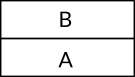
\includegraphics[width=0.35000\textwidth]{Figures/x86-ch/abcd-stack-step1.png}
\caption{A Stack with Two Values \lstinline!A! and \lstinline!B! Pushed
Respectively.}\label{fig:abcd-stack-step1}
\end{figure}

Let's assume that we have the string \lstinline!ABCD! and we would like
to push each character separately into the stack. First we start with
the operation \lstinline!push A! which puts the value \lstinline!A! on
the top of the stack, then we execute the operation \lstinline!push B!
which puts the value \lstinline!B! on top of the value \lstinline!A! as
we can see in the figure \ref{fig:abcd-stack-step1}, that is, the value
\lstinline!B! is now on the top of the stack and not the value
\lstinline!A!, the same is going to happen if we push the value
\lstinline!C! next as you can see in the figure
\ref{fig:abcd-stack-step2} and the same for the value of \lstinline!D!
and you can see the final stack of these four push operations in figure
\ref{fig:abcd-stack-step3}.

\begin{figure}
\centering
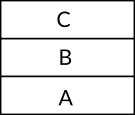
\includegraphics[width=0.35000\textwidth]{Figures/x86-ch/abcd-stack-step2.png}
\caption{A Stack with Three Values \lstinline!A!, \lstinline!B! and
\lstinline!C! Pushed Respectively.}\label{fig:abcd-stack-step2}
\end{figure}

\begin{figure}
\centering
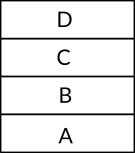
\includegraphics[width=0.35000\textwidth]{Figures/x86-ch/abcd-stack-step3.png}
\caption{A Stack with Four Values \lstinline!A!, \lstinline!B!,
\lstinline!C! and \lstinline!D! Pushed
Respectively.}\label{fig:abcd-stack-step3}
\end{figure}

Now let's assume that we would like to read the values from this stack,
the only way to read data in stack data structure is to use the
operation \lstinline!pop! which, as we have mentioned, removes the value
that resides on the top of the stack and returns it to the user, that
is, the stack data structure in contrary of array data structure
\footnote{Which is implemented by default in most major programming
  languages and know as arrays (in C for example) or lists (as in
  Python)} doesn't have the property of \emph{random access} to the
data, so, if you want to access any data in the stack, you can only use
\lstinline!pop! to do that. That means if you want to read the first
pushed value to the stack, then you need to \lstinline!pop! the stack
\lstinline!n! times, where \lstinline!n! is the number of pushed
elements into the stack, in other words, the size of the stack.

In our example stack, to be able to read the first pushed value which is
\lstinline!A! you need to \lstinline!pop! the stack four times, the
first one removes the value \lstinline!D! from the top of stack and
returns it to the user, which makes the values \lstinline!C! on the top
of stack as you can see in figure \ref{fig:abcd-stack-step2} and if we
execute \lstinline!pop! once again, the value \lstinline!C! will be
removed from the top of the stack and returns it to the user, which
makes the value \lstinline!B! on the top of the stack as you can see in
figure \ref{fig:abcd-stack-step1}, so we need to \lstinline!pop! the
stack two times more the get the first \lstinline!push!ed value which is
\lstinline!A!. This example makes it obvious for us why the stack data
structure is described as first-in-last-out data structure.

The stack data structure is one of most basic data structures in
computer science and there are many well-known applications that can use
stack to solve a specific problem in an easy manner. To take an example
of applications that can use a stack to solve a specific problem let's
get back to our example of \lstinline!push!ing \lstinline!ABCD! into a
stack, character by character and then \lstinline!pop!ping them back,
the input is \lstinline!ABCD! but the output of \lstinline!pop!
operation is \lstinline!DCBA! which is the reverse string of the input,
so, the stack data structure can be used to solve the problem of getting
the reversed string of an input by just pushing it into a stack
character by character and then popping this stack, concatenating the
returned character with the previously returned character, until the
stack becomes empty. Other problems that can be solved easily with stack
are palindrome problem and parenthesis matching problem which is an
important one for a part of programming languages' compilers and
interpreters known as parser.

As you can see in this brief explanation of stack data structure, we
haven't mention any implementation details which means that a specific
data structure is an abstract concept that describes a high-level idea
where the low-level details are left for the implementer.

\subsection{The Implementation: x86 Run-time
Stack}\label{the-implementation-x86-run-time-stack}

Now, with our understanding of the theoretical aspect of stack data
structure, let's see how the run-time stack is implemented in x86
architecture to be used for the objectives that we have mentioned in the
beginning of the subsection. As we have said earlier, the reason of x86
run-time stack's existence is to provide a way to implement function's
invocation, that is, the lifecycle of functions. Logically, we know that
a program consists of multiple functions (or \emph{routines} which is
another term that is used to describe the same thing) and when executing
a program (a process), a number of these functions (not necessarily all
of them) should be called to fulfill the required job.

In run-time context, a function \lstinline!B! starts its life when it's
called by another function \lstinline!A!, so, the function \lstinline!A!
is the \emph{caller}, that is, the function that originated the call,
and the function \lstinline!B! is the \emph{callee}. The caller can pass
a bunch of parameters to the callee which can reach the value of these
parameters while it's running, the callee can define its own local
variables which should not be reached by any other function, that means
that these variables can be removed from the memory once the callee
finishes its job. When the callee finishes its job, it may \emph{return}
some value to the caller \footnote{Some programming languages,
  especially those which are derived from Algol differentiate between a
  \emph{function} which \textbf{should} return a value to the caller,
  and a \emph{procedure} which \textbf{shouldn't} return a value to the
  caller.}. Finally, the run-time platform (the processor in the case of
compiled languages) should be able to know, when the callee finishes,
where is the place of the code that should be executed next, and
logically, this place is the line in the source code of the caller
function which is next to the line that called the callee in the first
place.

In x86, each process has its own run-time stack \footnote{We claim that
  for the purpose of explanation. But actually the matter of separated
  run-time stack for each process is a design decision that the
  operating system's kernel programmer/designer is responsible for.}, we
can imagine this run-time stack as a big (or even small, that depends on
practical factors) memory region that obeys the rules of stack data
structure. This run-time stack is divided into multiple mini-stacks,
more formally, these mini-stacks are called \emph{stack frames}. Each
stack frame is dedicated to \textbf{one} function which has been called
during the execution of the program, once this function exists, its
frame will be removed from the larger process stack, hence, it will be
removed from the memory.

The x86 register \lstinline!EBP! (which is called the \emph{stack frame
base pointer}) contains the starting memory address of the current stack
frame, and the register \lstinline!ESP! (which is called the \emph{stack
pointer}) contains the memory address of the top of the stack. To push a
new item into the run-time stack, an x86 instruction named
\lstinline!push! can be used with the value of the new item as an
operand, this instruction decrements the value of \lstinline!ESP! to get
a new \emph{starting} memory location to put the new value on and to
keep \lstinline!ESP! pointing to the top of the stack, decrementing the
value of \lstinline!ESP! means that the newly pushed items are stored in
a lower memory location than the previous value and that means the
run-time stack in x86 \emph{grows downward} in the memory.

When we need to read the value on the top of the stack and removes this
value from the stack, the x86 instruction \lstinline!pop! can be used
which is going to store the value (which resides on the top of stack) on
the specified location on its operand, this location can be a register
or a memory address, after that, \lstinline!pop! operation increments
the value of \lstinline!ESP!, so the top of stack now refers to the
previous value. Note that the \lstinline!pop! instruction only
increments \lstinline!ESP! to get rid of the popped value and don't
clear it from memory by, for example, writing zeros on its place which
is better for the performance, and this is one of the reasons when you
refer to some random memory location, for example in C pointers, and you
see some weird value that you probably don't remember that you have
stored it in the memory, once upon a time, this value may have been
pushed into the run-time stack and its frame has been removed. This same
practice is also used in modern filesystems for the sake of performance,
when you delete a file the filesystem actually doesn't write zeros in
the place of the original content of the file, instead, it just refer to
its location as a free space in the disk, and maybe some day this
location is used to store another file (or part of it), and this is when
the content of the deleted file are actually cleared from the disk.

Let's get back to x86 run-time stack. To make the matter clear in how
\lstinline!push! and \lstinline!pop! work, let's take an example. Assume
that the current memory address of the top of stack (\lstinline!ESP!) is
\lstinline!102d! and we executed the instruction \lstinline!push A!
where \lstinline!A! is a character encoded in \lstinline!UTF-16! which
means its size is \lstinline!2! bytes (\lstinline!16! bits) and it is
represented in hexadecimal as \lstinline!0x0410!, by executing this
\lstinline!push! instruction the processor is going to subtract
\lstinline!2! from \lstinline!ESP! (because we need to push
\lstinline!2! bytes into the stack) which gives us the new memory
location \lstinline!100d!, then the processor stores the first byte of
\lstinline!UTF-16! \lstinline!A! (\lstinline!0x04!) in the location
\lstinline!100d! and the second byte (\lstinline!0x10!) in the location
\lstinline!101d! \footnote{In fact, x86 is little-endian architecture
  which means that \lstinline!0x10! will be stored in the location
  \lstinline!100d! while \lstinline!0x04! will be stored in the location
  \lstinline!101d! but I've kept the example in the main text as is for
  the sake of simplicity.}, the value of \lstinline!ESP! will be changed
to \lstinline!100d! which now represents the top of the stack.

When we need to \lstinline!pop! the character \lstinline!A! from the top
of the stack, both bytes should be read and \lstinline!ESP! should be
\textbf{incremented} by \lstinline!2!. In this case, the new memory
location \lstinline!100d! can be considered as a \emph{starting}
location of the data because it doesn't store the whole value of
\lstinline!A! but a part of it, the case where the new memory location
is not considered as starting memory location is when the newly pushed
values is pushed as whole in the new memory location, that is, when the
size of this value is \lstinline!1! byte.

\subsection{Calling Convention}\label{calling-convention}

When a function \lstinline!A! needs to call another function
\lstinline!B!, then as a first step \lstinline!A! (the caller) should
push into the stack the parameter that should be passed to \lstinline!B!
(the callee), that means the parameters of \lstinline!B! will be stored
on the stack frame of \lstinline!A!, when pushing the parameters, they
are pushed in a reversed order, that is, the last parameter is pushed
first and so on. Then the x86 instruction \lstinline!call! can be used
to jump to function \lstinline!B! code. Before jumping to the callee
code, the instruction \lstinline!call! pushes the current value of
\lstinline!EIP! (this is, the returning memory address) onto the stack,
at this stage, the value of \lstinline!EIP! is the memory address of the
instruction of \lstinline!A! which is right after \lstinline!call B!
instruction, pushing this value into the stack is going to help the
processor later to decide which instruction of the running code should
be executed after the function \lstinline!B! finishes. Now, assume that
the function \lstinline!B! receives three parameters \lstinline!p1!,
\lstinline!p2! and \lstinline!p3!, the figure \ref{fig:call-conv-1}
shows the run-time stack at the stage where \lstinline!call! instruction
has been performed its first step (pushing \lstinline!EIP!). Also, the
following assembly code shows how \lstinline!A! pushes the parameters
then calls \lstinline!B!, as you can see, after \lstinline!B! finishes
and the execution of \lstinline!A! resumes, the value of \lstinline!EAX!
is moved to \lstinline!ECX! and this line is just an example and not a
part of calling convention.

\begin{lstlisting}
A:
; A's Code Before Calling B

push p3
push p2
push p1
call B
mov ecx, eax

; Rest of A's Code
\end{lstlisting}

\begin{figure}
\centering
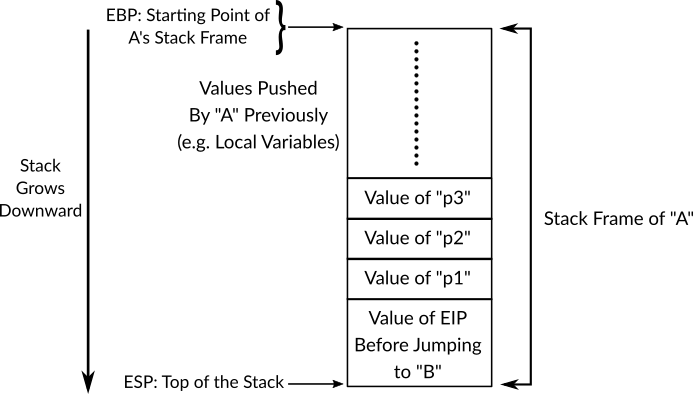
\includegraphics[width=0.55000\textwidth]{Figures/x86-ch/call-conv-1.png}
\caption{Run-time Stack Before Jumping to Function \lstinline!B!
Code}\label{fig:call-conv-1}
\end{figure}

When the processor starts executing function \lstinline!B!, or any other
function, it's the job of the function to create its own stack frame,
therefore, the first piece of any function's code should be responsible
for creating a new stack frame, this happens by moving the value of
\lstinline!ESP! (the memory address of the top of stack) to the register
\lstinline!EBP!, but before that, we should not lose the previous value
of \lstinline!EBP! (the starting memory address of the caller's stack
frame), this value will be needed when the callee \lstinline!B!
finishes, so, the function \lstinline!B! should push the value of
\lstinline!EBP! onto the stack and only after that it can change
\lstinline!EBP! to the value of \lstinline!ESP! which creates a new
stack frame for function \lstinline!B!, at this stage, both
\lstinline!EBP! and \lstinline!ESP! points to the top of the stack and
the value which is stored in the top of the stack is memory address of
the previous \lstinline!EBP!, that is, the starting memory location of
\lstinline!A!'s stack frame. Figure \ref{fig:call-conv-2} shows the
run-time stack at this stage. The following code shows the initial
instructions that a function should perform in order to create a new
stack frame as we just described.

\begin{lstlisting}
B:
push ebp
mov ebp, esp

; Rest of B's Code
\end{lstlisting}

\begin{figure}
\centering
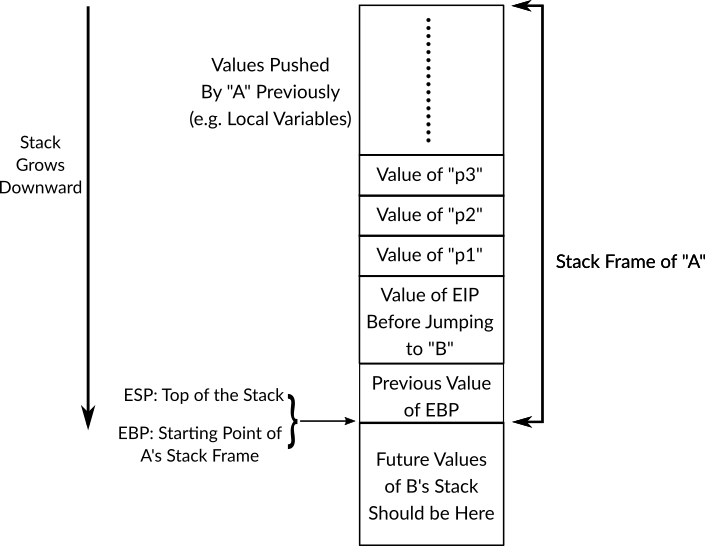
\includegraphics[width=0.55000\textwidth]{Figures/x86-ch/call-conv-2.png}
\caption{Run-time Stack After Jumping to Function \lstinline!B! Code and
Creating \lstinline!B!'s Stack Frame}\label{fig:call-conv-2}
\end{figure}

Now, the currently running code is function \lstinline!B! with its own
stack frame which contains nothing. Depending on \lstinline!B!'s code,
new items can be pushed onto the stack, and as we have said before, the
local variables of the function are pushed onto the stack by the
function itself, as you know, x86's protected mode is a
\lstinline!32-bit! environment, so, the values that are pushed onto the
stack through the instruction \lstinline!push! are of size \lstinline!4!
bytes (\lstinline!32! bits).

Pushing a new item will make the value of \lstinline!ESP! to change, but
\lstinline!EBP! remains the same until the current function finishes its
work, this will make \lstinline!EBP! too useful when we need to reach
the items that are stored in previous function's stack frame (in our
case \lstinline!A!), for example, the parameters or even the items that
are in the current function's stack frame but are not in the top of the
stack, as you know, in this case \lstinline!pop! cannot be used without
losing other values. Instead, \lstinline!EBP! can be used as a reference
to the other values. Let's take an example of that, given the run-time
stack in figure \ref{fig:call-conv-2} assume that function \lstinline!B!
needs to get the value of \lstinline!p1!, that can be achieved by
reading the memory location of the memory address \lstinline!EBP + 8!.
As you can see from the figure, memory address of \lstinline!EBP! points
to the previous value of \lstinline!EBP! which its size is \lstinline!4!
bytes, so if we add \lstinline!4! to the value in \lstinline!EBP!, that
is, \lstinline!EBP + 4! we will get the memory address of the location
which stores the resume point (\lstinline!EIP! before calling
\lstinline!B!) which also has the size of \lstinline!4! bytes, so, if we
add another \lstinline!4! bytes to \lstinline!EBP! we will reach the
item which is above the resume point, which will always (because the
convention always work the same way with any function) be the first
parameter if the current function receives parameters, and by adding
another \lstinline!4! to \lstinline!EBP! we will get the second
parameter and so on. The same is applicable if we would like to read
values in current function's stack frame (e.g.~local variables), but
this time we need to subtract from \lstinline!EBP! instead of adding to
it. Whether we are adding to or subtracting from \lstinline!EBP! the
value will always be \lstinline!4! and its multiples since each item in
x86 protected-mode run-time stack is of \lstinline!4! bytes. The
following assembly example of \lstinline!B! reads multiple values from
the stack that cannot be read with normal \lstinline!pop! without
distorting the stack.

\begin{lstlisting}
B:
; Creating new Stack Frame
push ebp
mov ebp, esp

push 1 ; Pushing a local variable
push 2 ; Pushing another local variable

; Reading the content 
; of memory address EBP + 4
; which stores the value of
; the parameters p1 and moving
; it to eax.
mov eax, [ebp + 8]

; Reading the value of the
; first local varaible and
; moving it to ebx.
mov ebx, [ebp - 4]

; Rest of B's Code
\end{lstlisting}

When \lstinline!B! finishes and needs to return a value, this value
should be stored in the register \lstinline!EAX!. After that,
\lstinline!B! should deallocates its own stack frame, this task can be
accomplished easily by popping all values of \lstinline!B!'s stack frame
until we reach to first value pushed value by \lstinline!B! (the
starting memory address of the caller \lstinline!A! stack frame) which
should be set to \lstinline!EBP! in order to restore the stack frame of
\lstinline!A! as the current stack frame. After that, the top of the
stack contains the returning memory address which should be loaded to
\lstinline!EIP! so we can resume the execution of the caller
\lstinline!A!, that's can be done by using the x86 instruction
\lstinline!ret! which pops the stack to get the returning address then
loads \lstinline!EIP! with this value. Finally, when \lstinline!A! gains
the control again it can deallocate the parameters of \lstinline!B! to
save some memory by just popping them. The method that we have described
to deallocate the whole stack frame or deallocate the parameters is the
standard way that's not widely used practically for multiple reasons,
one of these reasons is that \lstinline!pop! needs a place to store the
\lstinline!pop!ped value, this place can be a register or a memory
location, but what we really need is to get rid of these values, so,
storing them in another place is a waste of memory. In order to explain
the other way of deallocating some items from the stack consider the
following code:

\begin{lstlisting}
sub esp, 4
mov [esp], 539
\end{lstlisting}

This code is equivalent to \lstinline!push 539!, it does exactly what
\lstinline!push! does, first it subtract \lstinline!4! bytes from top of
stack's memory address to get a new memory location to store the new
value in, then, it stores the value in this location. The reverse
operation is performed with \lstinline!pop! as the following which is
equivalent to \lstinline!pop eax!.

\begin{lstlisting}
mov eax, [esp]
add esp, 4
\end{lstlisting}

As you can see, to get rid of the \lstinline!pop!ped value, only top of
stack's memory address has been changed. Since every item on the stack
is of size \lstinline!4! bytes, then adding \lstinline!4! to
\lstinline!ESP! makes it point to the item which is exactly above the
current one in the stack. So, if we need to get rid of the value on the
top of stack without getting its value and storing it somewhere else, we
can simply use the following instruction \lstinline!add esp, 4!. What if
we want to get rid of the value on the top of the stack and the value
before it? The total size of both of them is \lstinline!8! bytes, so,
\lstinline!add esp, 8! will do what we want. This technique is
applicable for both deallocating \lstinline!B!'s stack frame and its
parameters from \lstinline!A!'s stack frame. For the former, there is a
yet better technique. In order to deallocate the stack frame of the
current function we can simply do the following:
\lstinline!mov esp, ebp!, that is, move the memory address of
\lstinline!EBP! to \lstinline!ESP!, which was the state when the callee
\lstinline!B! just started. The following is the last part of
\lstinline!B! which deallocates its own stack frame and return to
\lstinline!A!.

\begin{lstlisting}
B:
; Previous B's Code:
;        Creating new Stack Frame
;        Pushing Local variable
;        The Rest of Code

; Make to the of stack points
; to the first value pushed
; by the function "B".
mov esp, ebp

; Pop the current top of
; stack and put the value
; in "EBP" to make A's
; stack frame as the current.
pop ebp

; Jump the the resume point.
ret
\end{lstlisting}

The details of calling a function that we have just described are
\textbf{implementation details} and we mentioned previously that these
implementation details of function's invocation are known as calling
conventions. The calling convention that we have described is known as
\lstinline!cdecl! which stands for \emph{C declaration}, there are other
conventions, which means the one which we have described is not an
strict standard for x86 architecture, instead, the operating systems,
compilers and low-level code writers can decide which calling convention
that they would like to use or maybe make up a wholly new one according
to their objective. However, the reason behind choosing
\lstinline!cdecl! to explain here is that it is a well-known and widely
used calling convention, also, it serves our purpose of explaining the
basics of x86 run-time stack.

\subsection{Growth Direction of Run-time
Stack}\label{growth-direction-of-run-time-stack}

When we explained how x86 instructions \lstinline!push! and
\lstinline!pop! work, we have claimed that the x86 run-time stack
\emph{grows downward}, so, what does growing downward or upward exactly
means? Simply, when we said that x86 run-time stack grows downward we
meant the the older items of stack are pushed on larger memory addresses
while the most recent ones are pushed onto smaller memory addresses. For
example, starting from the memory address \lstinline!104d!, let's assume
we have pushed the value \lstinline!A! after that we pushed the value
\lstinline!B!, then \lstinline!A!'s memory location will be
\lstinline!104d! while \lstinline!B!'s memory location will be
\lstinline!100d!, so the new values will always be pushed on the bottom
of the old ones in the memory.

\begin{figure}
\centering
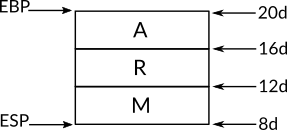
\includegraphics[width=0.35000\textwidth]{Figures/x86-ch/Fig10062021_0.png}
\caption{An Example of a Run-Time Stack with Three
Items}\label{fig:10062021_0}
\end{figure}

What makes we claim that, for instance, the address \lstinline!100d! is
at the bottom of \lstinline!104d! instead of the other way around is how
we visualize the run-time stack inside the main memory. Let's look at
the figure \ref{fig:10062021_0} which shows a run-time stack that
contains three items \lstinline!M!, \lstinline!R! and \lstinline!A! and
all of them are of \lstinline!4! bytes, on the right side of the figure
we can see the starting memory address of each item. As we can see, in
this visualization of the run-time stack, the smaller memory addresses
are on the bottom and the larger memory addresses are on the top.

From the figure we can see that the value of \lstinline!ESP! is
\lstinline!8d! \footnote{As a reminder, don't forget that all these
  memory address are actually \textbf{offsets} inside a stack segment
  and not a whole memory address.}, let's assume that we would like to
run the instruction \lstinline!push C! on this run-time stack, as we
have mentioned before, the instruction \lstinline!push! of x86 is going
to decrease the value of \lstinline!ESP! by a size decided by the
architecture (\lstinline!4! bytes in our case) in order to get a new
starting memory address for the new item. So, \lstinline!push! is going
to subtract \lstinline!4d! (The size of pushed item \lstinline!C! in
bytes) from \lstinline!8d! (current \lstinline!ESP! value) which gives
us the new starting memory location \lstinline!4d! for the item
\lstinline!C!. If we visualize the run-time stack after pushing
\lstinline!C! it will be the one as on figure \ref{fig:10062021_1} and
we can see, depending on the way of \lstinline!push! instruction works,
that the stack grew downwards by pushing the new item \lstinline!C! on
the bottom. So, according to this visualization of run-time stack, which
puts larger memory addresses on the top and smaller on the bottom, we
can say x86 run-time stack grows downward \emph{by default}.

\begin{figure}
\centering
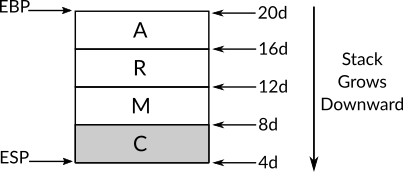
\includegraphics[width=0.35000\textwidth]{Figures/x86-ch/Fig10062021_1.png}
\caption{A New Item Pushed Into a Stack that Grows
Downward}\label{fig:10062021_1}
\end{figure}

This visualization is just one way to view how the run-time stack grows,
which means they may be other visualizations, and the most obvious one
is to reverse the one that we just described by putting the smaller
addresses on the top and the larger addresses on the bottom as shown in
figure \ref{fig:10062021_2}, you can note that in contrast to figure
\ref{fig:10062021_1} the smallest address \lstinline!4d! is on top, so,
based on this visualization the stack grows upward! Actually this latter
visualization of run-time stack is the one which is used in Intel's
manual and the term \emph{expand-up} is the term that is used in the
manual to describe the direction of stack growth.

\begin{figure}
\centering
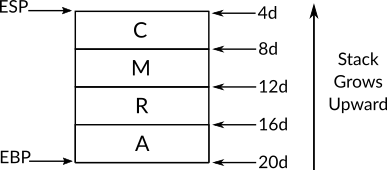
\includegraphics[width=0.35000\textwidth]{Figures/x86-ch/Fig10062021_2.png}
\caption{A Stack that Grows Upward Instead of
Downward}\label{fig:10062021_2}
\end{figure}

To sum it up, the direction in which the run-time stack grows (down or
up) depends on how do you visualize the run-time stack, as in figure
\ref{fig:10062021_1} or as in figure \ref{fig:10062021_2}. In our
discussion in this book we are going to depend on the first
visualization\footnote{And many other books actually uses the first
  visualization as I recall and for that I chose it in this book. And
  according to my best knowledge the only reference that I've seen that
  depends on the second visualization is Intel's manual.}, so, simply,
the run-time stack of x86 grows downward.

\subsection{The Problem of Resizing the Run-time
Stack}\label{the-problem-of-resizing-the-run-time-stack}

We have emphasized that x86 run-time stack \textbf{by default} grows
downward, this default behavior can be changed if we wish to, which is
going to make the run-time stack to grow upwards instead and the way to
do that is to use expansion-direction flag of run-time stack's segment
descriptor, we have mentioned this flag when explained the structure of
segment descriptor and postponed its details till here.

When we want the run-time stack to grow downward (or in Intel's term
which depends on the second visualization of run-time stack:
\textbf{expand-up}) the value of this flag should be \lstinline!0!, on
the other hand, when we want the run-time stack to grow upward (in
Intel's term: \textbf{expand-down}) the value of this flag should be
\lstinline!1!. Modern operating systems use the default behavior
(downward growth), we will see that this design decision is taken due to
the choice of flat memory model by modern operating systems. However,
the other available option (upward growth) is there to solve a potential
problem and whether this problem is going to show up in a specific
kernel depends on how this kernel's architecture is designed, that is,
which memory model is used in this kernel.

This problem, which we can solve by making the run-time stack grows
upward instead of downward, is related to the need of increasing the
size of run-time stack and the fact that the run-time stack stores
memory addresses \footnote{The previous values of \lstinline!EBP! and
  \lstinline!EIP!. Also the application programmer may store memory
  addresses of local variables in the stack (e.g.~by using pointers in
  C).} on it. Let's assume that our kernel created a new stack segment
for a specific process \lstinline!X! and this stack segment has a fixed
size which is \lstinline!50! bytes \footnote{As you may recall, the size
  of the segment can be decided by the base address of the segment and
  its limit as specified in the segment's descriptor.} for example. The
process \lstinline!X! starts its work and at some point of time its
run-time stack of size \lstinline!50! bytes becomes full which means
that we need to resize it and make it bigger so it can hold more items,
let's assume the new size will be \lstinline!60! bytes.

\begin{figure}
\centering
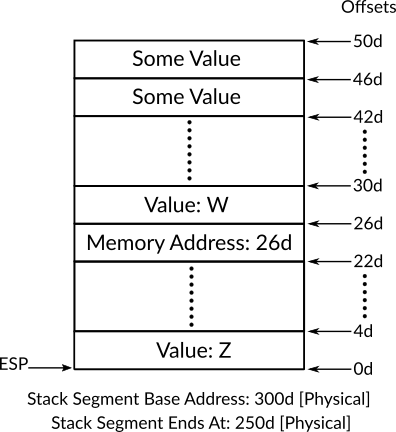
\includegraphics[width=0.35000\textwidth]{Figures/x86-ch/Fig10062021_3.png}
\caption{Process X's Run-time Stack}\label{fig:10062021_3}
\end{figure}

Before going any further with our discussion, let's see the figure
\ref{fig:10062021_3} which represents a snapshot of process
\lstinline!X!'s run-time stack when it became full. We can see from the
figure that \lstinline!X!'s stack segment starts from the
\textbf{physical} memory address \lstinline!300d! (segment's base
address) and ends at the \textbf{physical} memory address
\lstinline!250d!, also, the items of run-time stack are referred to
based on their offsets inside the stack segment. We can see that a bunch
of values have been pushed onto the stack, some of those values are
shown on the figure and some other are omitted and replaced by dots
which means that there are more values here in those locations. Normal
values are called ``some value'' in the figure and the last pushed value
in the stack is the value \lstinline!Z!. Also, a value which represents
a \textbf{logical memory address} has been pushed onto the stack, more
accurately, this value represents an \textbf{offset} within the current
stack segment, a \textbf{full} logical memory address actually consists
of both offset \textbf{and} segment selector as we have explained
earlier in this chapter when we discussed address translation. But for
the sake of simplicity, we are going call this stored value as ``memory
address'' or ``memory location'' in our current explanation. As we
explained earlier, all memory addresses that the processes work with are
logical and not physical. The value \lstinline!26d! is a local variable
\lstinline!P! of the type pointer (as in C) which points to another
local variable \lstinline!R! that has the value \lstinline!W! and is
stored in the memory location \lstinline!26d!.

\begin{figure}
\centering
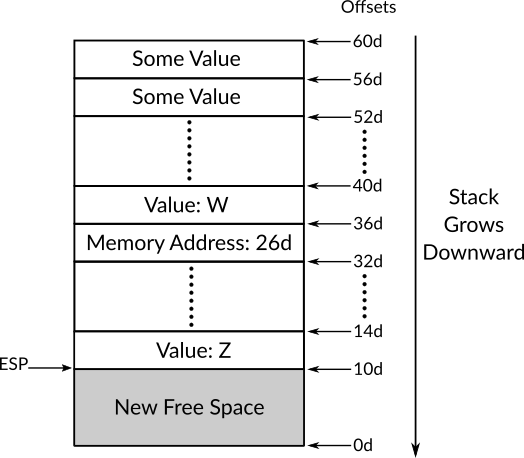
\includegraphics[width=0.35000\textwidth]{Figures/x86-ch/Fig10062021_4.png}
\caption{Process X's Run-time Stack After Resize (Grows
Downward)}\label{fig:10062021_4}
\end{figure}

Figure \ref{fig:10062021_4} shows \lstinline!X!'s stack after resize, as
you can see we have got our new free space of \lstinline!10! bytes,
also, because the stack grows downward so the new free space should be
added on the bottom of the stack to be useful which means the previous
offsets should be changed, therefore, the largest offset \lstinline!50d!
has been updated to \lstinline!60d! by adding \lstinline!10d! (which is
the newly added free space to the stack in bytes) to it and so on for
the rest of offsets, also, \lstinline!ESP! has been simply updated in
the same manner.

Now we can see that the process of updating the offsets, that we are
forced to perform because the stack grows downward, has caused a problem
in the offsets which have been pushed onto the stack before resizing it.
You can see the pointer \lstinline!P! which still has the original value
\lstinline!26d!, that means it doesn't point the the variable
\lstinline!R! anymore, instead it is going to point to another memory
location now with a value other than \lstinline!W!, and the same problem
holds for all pushed \lstinline!EBP! values on \lstinline!X!'s stack.

A potential solution for this problem is to update all stack items that
contain memory addresses in the range of the stack after resizing it,
exactly as we have done with \lstinline!EBP!, but more simpler solution
is to make the stack to grow upwards instead of downwards! Modern
operating systems solves this problem by not dividing the memory into
segments but they use flat memory model which views the memory as one
big segment for all data, code and stacks.

\begin{figure}
\centering
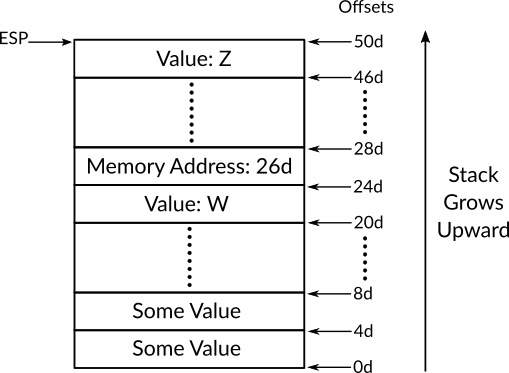
\includegraphics[width=0.35000\textwidth]{Figures/x86-ch/Fig12062021_1.png}
\caption{Process X's Run-time Stack (Grows
Upward)}\label{fig:12062021_1}
\end{figure}

Now let's see what happens in the same scenario but with changing the
growth direction of the stack from downward which caused the problem to
upwards. In this case, as we have said before, the new items will be
stored on the larger memory addresses (offsets to be more accurate).
Figure \ref{fig:12062021_1} shows the same snapshot of \lstinline!X!'s
run-time of stack as in the one of figure \ref{fig:10062021_3} but this
time it grows upwards instead of downward. You can notice that the older
values are now on the bottom of the stack, that is, on smaller memory
addresses, what interests us in this stack is the entry which stores the
memory address \lstinline!20d! that points to the memory location which
has the value \lstinline!W! and it is the one which caused the problem
in the first place. When the stack was growing downward, the memory
location of the value \lstinline!W! was \lstinline!26d!, but this time
it is \lstinline!20d!. So, what happens when we need to resize this
run-time stack?

In the same way of the previous one, the limit of the stack (its largest
offset) will be increased from \lstinline!50d! to \lstinline!60d! as
shown in figure \ref{fig:12062021_2}, but in contrast to the previous
one, we don't need to update the value of \lstinline!ESP! anymore,
because as you can see from the two figures \ref{fig:12062021_1} and
\ref{fig:12062021_2} the memory address \lstinline!50d! represents the
top of the stack on both stacks. The same holds true for the stack item
which stores the memory address \lstinline!20d!, we don't need to update
it because the value \lstinline!W! is still on the same memory address
(offset) and can be pointed to by the memory address \lstinline!20d!.
So, we can say that deciding the direction of run-time stack growth to
be upward instead of downward can easily solve the problem of getting
wrong stored memory address after resizing the run-time stack \footnote{Actually,
  the well-know stack overflow vulnerability in x86 is also caused by
  stack growing downward and can be avoided easily in growing upwards
  stacks!} and that's when we use segmentation as a way of viewing the
memory.

\begin{figure}
\centering
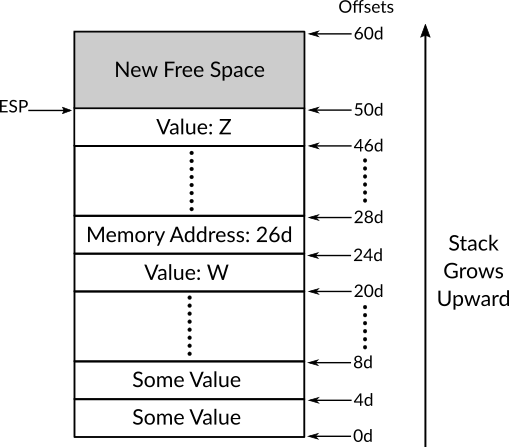
\includegraphics[width=0.35000\textwidth]{Figures/x86-ch/Fig12062021_2.png}
\caption{Process X's Run-time Stack (Grows Upward)
Resized}\label{fig:12062021_2}
\end{figure}

\section{x86 Interrupts}\label{x86-interrupts}

Event-driven programming is a common programming paradigm that is used
in many areas of programming. One of these areas is graphical user
interface (GUI) programming, also, it is common in game development,
furthermore, some network programming frameworks use this paradigm. In
this paradigm, the program is driven by \emph{events}, that is, it keeps
idle and waiting for any even to occur and once an event occurs the
program starts to work by handling this event, for example, a mouse
click is considered as an event in GUI programming. When an event
occurs, the program handles this event through, usually, a separated
function which is dedicated for this event, this function is known as a
\emph{handler}. In GUI programming for example, when the user clicks on
a specific button, that is, when this event occurs, a function specified
for this event on this button (the handler) is called to perform some
operation after this click, such as, save a document or close the
application.

This paradigm is also used by x86. When a process is running, something
can \emph{interrupt} (an event occurred) the processor which is going,
in this case, to stop the execution of the current process temporarily,
and call the suitable \emph{interrupt handler} (also called
\emph{interrupt service routine}) to handle the current interrupt, after
handling the interrupt, the processor can resume the process which was
running before the interrupt occurred.

One example of the usage of interrupts in this low-level environment is
the \emph{system timer}. In the hardware level, there could be a system
timer which interrupts the processor in each \lstinline!X! period of
time and this type of interrupt is the one that makes multitasking
possible in uniprocessor systems. When a processor is interrupted by the
system timer, it can call the kernel which can change the currently
running process to another one; this operation known as
\emph{scheduling} which its goal is distributing the time of the
processor to the multiple processes in the system.

Another example of using interrupts is when the user of an operating
system presses some keys on the keyboard, these events of pressing
keyboard keys should be sent to the kernel which is going to delegate
the \emph{device driver} \footnote{That's why in some kernel's designs,
  especially, monolithic kernel keeps the device drivers as a part of
  the kernel.} of the keyboard to handle these events in a proper way,
in this case, with each key press, the keyboard is going to interrupt
the processor and request to handle these events.

In x86, both hardware and software can interrupt the processor, system
timer and keyboard are examples of \emph{hardware interrupts} while the
\emph{software interrupt} can occur by using the x86 instruction
\lstinline!int! which we have used when we wrote our bootloader, the
operand of this instruction is the \emph{interrupt number}, for example,
in our bootloader we have used the following line \lstinline!int 10h!,
in this case, the interrupt number is \lstinline!10h! (\lstinline!16d!)
and when the processor is interrupted by this instruction, it is going
to call the handler of interrupt number \lstinline!10h!. Software
interrupt can be used to implement what is known as \emph{system calls}
which provide a way for user applications to call a specific kernel's
code that gives the applications some important services such as
manipulating the filesystem (e.g.~reading or writing files, create new
file or directories, etc.) or creating new process and so on in a way
that resembles the one that we used to call BIOS services.

In addition to interrupts, \emph{exceptions} can be considered as
another type of events which also stop the processor from its current
job temporarily and make it handle it and then resume its job after
that. The main difference between exceptions and interrupts in x86 is
that the former occurs when an error happens in the environment, for
example, when some code tries to divide some number by zero, an
exception will be generated and some handler should do something about
it, we can perceive the exceptions of x86 as the exceptions of some
programming languages such as C++ and Java.

\subsection{Interrupt Descriptor
Table}\label{interrupt-descriptor-table}

In x86, there is a table known as \emph{interrupt descriptor table}
(\lstinline!IDT!), also may called \emph{interrupt vector table} but the
term that Intel uses is the former one while the latter are used to
describe this kind of tables as a concept in some works of literature
and not the name of the table on a specific architecture.
\lstinline!IDT! resides in the memory and tells the processor how to
reach to the handler of a given interrupt number. The entries of
\lstinline!IDT! are known as \emph{gate descriptors} and the size of
each one of them is \lstinline!8! bytes same as \lstinline!GDT! and
\lstinline!LDT!. At most, \lstinline!IDT! can contain \lstinline!256!
gate descriptors and the base memory address of \lstinline!IDT! is
stored in a special register known as \lstinline!IDTR!.

\begin{figure}
\centering
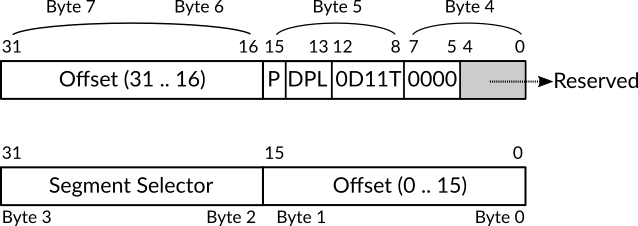
\includegraphics[width=0.50000\textwidth]{Figures/x86-ch/Fig210621_0.png}
\caption{Gate Descriptor Structure for Interrupt and Trap
Gates}\label{fig:210621_0}
\end{figure}

The gate descriptors in the \lstinline!IDT! table can be of three types,
\emph{task gate}, \emph{interrupt gate} and \emph{trap gate}, our focus
currently will be on the latter two. The structure of both interrupt and
trap gate descriptor is shown in figure \ref{fig:210621_0}. As we have
said earlier, a gate descriptor of the \lstinline!IDT! should point to
the memory address of the interrupt handler's code. We can see in the
figure that bytes \lstinline!2! and \lstinline!3! should contain a
segment selector, which is the segment selector of handler's code, that
is, the index of the code segment that contains handler's code, we can
see an important difference between \lstinline!GDT! and \lstinline!IDT!
here. In the former the base address of a segment is a linear address,
while the base address of the handler is a logical address.

The offset of the first handler's instruction should be set in the
descriptor, this will be useful if the handler's code is just a part of
the whole code segment which is presented in the segment selector field.
The offset in the gate descriptor is divided into two parts, the least
significant\lstinline!2! bytes of the offset should be loaded into bytes
\lstinline!0! and \lstinline!1! of the descriptor, while the most
significant\lstinline!2! bytes of the offset should be loaded into bytes
\lstinline!6! and \lstinline!7!.

The least significant nibble of byte \lstinline!4! is reserved and the
most significant nibble of byte \lstinline!4! should always be
\lstinline!0d!. The most significant bit of byte \lstinline!5! is
present flag (\lstinline!P! flag), when its value is \lstinline!0! that
means the code that this descriptor is pointing to is not loaded into
memory, while the value \lstinline!1! means otherwise. The descriptor
privilege level field (\lstinline!DPL!) contains the privilege level of
the handler, it occupies the second and third least significant bit of
byte \lstinline!5!. The value of fourth, sixth and seventh least
significant bits of byte \lstinline!5! should always be \lstinline!0b!,
\lstinline!1b! and \lstinline!1b! respectively. The flag which is called
\lstinline!D! in the figure specifies the size of the gate descriptor
itself whether it is \lstinline!32! bits, when\lstinline!D! flag =
\lstinline!1!, or \lstinline!16! bits when \lstinline!D! flag =
\lstinline!0!, the former should always be our choice in protected-mode,
while the latter should always be our choice in real-mode. The flag
which is called \lstinline!T! in the figure specifies whether the gate
is an interrupt gate, when \lstinline!T! flag = \lstinline!0!, or the
gate is an trap gate, when \lstinline!T! flag = \lstinline!1!.

The difference between interrupt and trap gates is too simple, when a
handler defined as an interrupt gate is called, the processor is going
to disable the ability to signal a new interrupt until the handler
returns, that is, the execution of the handler will not interrupted
until it finishes its job and return to the caller, of course there are
some exceptions, a type of interrupts known as \emph{non-maskable
interrupts} (\lstinline!NMI!) will interrupt the execution of the
current code even if the interruption is disabled, non-maskable
interrupts occur when some catastrophic event (from the hardware
perspective) happens in the system. On the other hand, the handler that
is defined as a trap gate can be interrupted by any new interrupt, that
is, the interruption will not be disabled by the processor.

However, disabling interruption is an operation that can be performed by
the code by using the x86 instruction \lstinline!cli! (still,
non-maskable interrupts are excepted) which stands for \emph{clear
interrupt flag} and can be enabled again by using the instruction
\lstinline!sti! which stands for \emph{set interrupt flag}, both of
these instructions manipulate the value of \emph{interrupt flag} which
is a part of the register \lstinline!EFLAGS!.

Now, let's assume that we have defined a gate descriptor for a handler,
let's name it \lstinline!A!. The question is, which interrupt the
handler \lstinline!A! is going to handle? In other words, for which
interrupt number the processor is going to call the code of
\lstinline!A! to handle the interrupt? In fact, that depends on the
index of \lstinline!A!'s gate descriptor in the \lstinline!IDT! table.
Let's assume that the index is \lstinline!0d!, then \lstinline!A!'s code
will be called when the interrupt number \lstinline!0! is signaled, that
means the term interrupt number is a synonym for entry's index number in
\lstinline!IDT! table

In protected-mode, interrupt numbers, that is \lstinline!IDT! entries
indices, from \lstinline!0! to \lstinline!21! have specific meaning
defined by x86 architecture itself, for example, the interrupt number
that is reserved for division by zero exception is the interrupt number
\lstinline!0! and, in our example, the code of \lstinline!A! will be
called when some other code divides a number by zero. Beside interrupt
numbers \lstinline!0! to \lstinline!21!, the range of interrupts number
from \lstinline!22! to \lstinline!31! are reserved, and the interrupt
numbers from \lstinline!32! to \lstinline!255! are available for the
system programmer to decide their meanings, however, not all of their
descriptors should be filled, only the needed ones will be enough.

\subsubsection{\texorpdfstring{The Register
\texttt{IDTR}}{The Register IDTR}}\label{the-register-idtr}

In same way as \lstinline!GDT!, we should tell the processor where the
\lstinline!IDT! reside in the memory and that can be performed by the
instruction \lstinline!lidt! which stands for \emph{l}oad
\lstinline!IDT!, this instructions works as \lstinline!lgdt!, it takes
an operand and loads it to the register \lstinline!IDTR! which will be
used later by the processor to reach to the \lstinline!IDT! table.

The structure of \lstinline!IDTR! is same as \lstinline!GDTR!, its size
is \lstinline!48! bits and it's divided into two parts, the first part
represents the size of the \lstinline!IDT! in bytes, that is, the
\lstinline!IDT!'s limit, this field starts from bit \lstinline!0! of
\lstinline!IDTR! and ends at bit \lstinline!15!. Starting from bit
\lstinline!16! up to bit \lstinline!47! the base linear address
\footnote{As we have mentioned multiple time that in our current case,
  where the paging is disabled, a linear address is same as physical
  address.} where \lstinline!IDT! is reside should be set.
